\documentclass{tufte-handout}

\title{STAT 24410 Lecture Notes}

\author{Marcus Kuo}

\date{\today} % without \date command, current date is supplied

%\geometry{showframe} % display margins for debugging page layout

\usepackage{lastpage} % Required to determine the last page number for the footer
\usepackage{enumerate}
\usepackage{amssymb}
\usepackage{verbatim}
\usepackage{mathrsfs}
\usepackage[most]{tcolorbox} % Required for boxes that split across pages
\usepackage{booktabs} % Required for better horizontal rules in tables
\usepackage{listings} % Required for insertion of code
\usepackage{etoolbox} % Required for if statements
\usepackage{mathrsfs}
\usepackage{amssymb}
\usepackage{capt-of}
\usepackage{soul}
\usepackage{pdfpages}
\usepackage{xcolor}
\usepackage{hyperref}
\usepackage{graphicx} % allow embedded images
\setkeys{Gin}{width=\linewidth,totalheight=\textheight,keepaspectratio}
\graphicspath{{}} % set of paths to search for images
\usepackage{amsmath}  % extended mathematics
\usepackage{booktabs} % book-quality tables
\usepackage{units}    % non-stacked fractions and better unit spacing
\usepackage{multicol} % multiple column layout facilities
\usepackage{lipsum}   % filler text
\usepackage{fancyvrb} % extended verbatim environments
\fvset{fontsize=\normalsize}% default font size for fancy-verbatim environments
\usepackage{amsthm}
\usepackage{centernot}
\usepackage{dsfont}
\usepackage{tikz}
\usepackage{pgfplots}

% Standardize command font styles and environments
\newcommand{\doccmd}[1]{\texttt{\textbackslash#1}}% command name -- adds backslash automatically
\newcommand{\docopt}[1]{\ensuremath{\langle}\textrm{\textit{#1}}\ensuremath{\rangle}}% optional command argument
\newcommand{\docarg}[1]{\textrm{\textit{#1}}}% (required) command argument
\newcommand{\docenv}[1]{\textsf{#1}}% environment name
\newcommand{\docpkg}[1]{\texttt{#1}}% package name
\newcommand{\doccls}[1]{\texttt{#1}}% document class name
\newcommand{\docclsopt}[1]{\texttt{#1}}% document class option name
\newcommand{\verteq}[0]{\begin{turn}{90} $=$\end{turn}}

\newcommand*\N{\mathbb{N}}
\newcommand*\R{\mathbb{R}}
\newcommand*\Q{\mathbb{Q}}
\newcommand*\Z{\mathbb{Z}}
\newcommand*\E{\mathbb{E}}
\let\oldP\P
\renewcommand{\P}{\mathbb{P}}
\let\O\varnothing
\let\oldemptyset\emptyset
\let\emptyset\varnothing

\DeclareMathOperator*{\argmax}{arg\,max} % thin space, limits underneath in displays
\DeclareMathOperator*{\argmin}{arg\,min} % thin space, limits underneath in displays

\newenvironment{docspec}{\begin{quote}\noindent}{\end{quote}}% command specification environment

\newtheorem{thm}{Theorem}[subsection]
\newtheorem{lemma}[thm]{Lemma}
\newtheorem{cor}[thm]{Corollary}
\newtheorem{rmk}[thm]{Remark}
\newtheorem{conj}[thm]{Conjecture}
\newtheorem{ex}[thm]{Example}
\newtheorem{aside}[thm]{Aside}
\newtheorem{notation}[thm]{Notation}
\newtheorem{prop}[thm]{Proposition}

\theoremstyle{definition}
\newtheorem{defn}[thm]{Definition}

\setcounter{secnumdepth}{2}
\setcounter{tocdepth}{1}

\begin{document}

\maketitle
\tableofcontents

\newpage

\section{Course Motivation: Genome-wide Association Studies}

An overview of the course content.

\section{Introduction to Probability and Random Variables}

\subsection{Probability Spaces, Conditional Probability, Independence}

\begin{notation}
	Let $\Omega$ be a sample space (set of points). Subsets of $\Omega$ are called events and elements in $\Omega$ are called sample points.
\end{notation}
\begin{defn}[$\sigma$-field]
	A $\sigma$-field $\mathscr{F}$ is a collection of events such that:
	\begin{enumerate}[(i)]
		\item $\Omega \subseteq \mathscr{F}$
		\item $A \subseteq \mathscr{F} \implies A^c \subseteq \mathscr{F}$
		\item $\{A_n\} \subseteq \mathscr{F} \implies \bigcup\limits_{n}^{}  A_n \subseteq \mathscr{F}$.
	\end{enumerate}
	The Borel set $\mathscr{B}$ is the smallest $\sigma$-field that contains all open intervals $(a,b)$ for $\Omega = R$.
\end{defn}

\begin{defn}[Probability measure]
	Suppose we have $(\Omega, \mathscr{F}).$ A probability measure $P: \mathscr{F} \to [0,1]$ has the following properties:
	\begin{enumerate}[(i)]
		\item $\P(\Omega) = 1$
		\item $\P\left( \bigcup\limits_{n}^{} A_n \right) = \sum\limits_{n} \P(A_n)$ if $A_i \cap A_j \ne \O$ for all $i \ne j$
	\end{enumerate}
\end{defn}

\begin{defn}[Random variable]
	A random variable $X: \Omega \to \R$ on $(\Omega, \mathscr{F}, P)$ is a function such that for every $B \in \mathscr{B}$, $X^{-1}(B) \subseteq \mathscr{F}$.
\end{defn}

\begin{defn}[Independence of random variables]
	The random variables $X$ and $Y$ are independent if \[
		\P\left[X \cap Y\right] = \P\left[x\right] \P\left[Y\right] 
	.\] 
\end{defn}



\begin{ex}
	Consider $(\Omega_1, \mathscr{F}_1, P_1)$ where $\Omega_1 = \{H, T\}$, $\mathscr{F}_1$ is all subsets of $\Omega_1$, and $P_1(\{H\}) = P_2(\{T\}) = \frac{1}{2}$. \\ Define $X_1(w) = \begin{cases}
		1, \quad w = H \\ 0, \quad w = T
	\end{cases}$.
\end{ex}

\begin{ex}
	Consider $(\Omega_2, \mathscr{F}_2, P_2)$ where $\Omega_2 = [0,1]$, $\mathscr{F}_2 = \mathscr{B}$, and $P_2\left( [a,b] \right) = b-a$.

	Define $X_2 = \begin{cases}
		1, \quad w \in [0,\frac{1}{2}] \\
		0, \quad w \in (\frac{1}{2}, 1]
	\end{cases}$.
\end{ex}

Although the spaces are totally different in these two examples, their distributions are identical. From now on, we don't care so much about the generation behind the distribution; the distribution itself is what's important.

\begin{defn}[Equal distributions]
	The random variables $X_1, X_2$ are equal in distribution if \[
		\P(X_1 \in A) = \P(X_2 \in A)
	\] for all $A$.
\end{defn}

Next time, we will relate this definition to the CDF.


\subsection{The Cumulative Distribution Function}
\begin{defn}[Cumulative distribution function]
	Let $X$ be a random variable. The cumulative distribution function of $X$ denoted by $F$ or $F_x$ dis a function $F: \R \to [0,1]$ such that \[
		F(x) = \P\left[X \in (-\infty, x] \right] = \P\left[X \le x \right] 
	.\] 		
\end{defn}

\begin{lemma}
	Two random variables $X,Y$ have the same distribution ($X =_{\mathscr{D}} Y$) if and only if \[
		F_X(t) = F_Y(t)
	\] for every $t \in \R$.
\end{lemma}

\begin{proof}
	The forwards direction is immediate and the backwards direction requires constructing a set from open intervals.
\end{proof}

\begin{ex}
	$\text{Binomial}(2, \frac{1}{2})$ has a discrete CDF: \[
		F(x) = \begin{cases}
			0, \quad &x \in (-\infty,0) \\
			\frac{1}{4}, \quad &x \in [0, 1) \\
			\frac{3}{4}, \quad &x \in [1,2) \\
			1, \quad &x \in [2,\infty)
		\end{cases}
	.\] 
\end{ex}

\begin{ex}
	$\text{Uniform}(0,1)$ has a continuous CDF:
	\[
		F(x) = \begin{cases}
			0, \quad &x \in (-\infty,0) \\
			x, \quad &x \in [0,1] \\
			1, \quad &x \in (1,\infty)
		\end{cases}
	.\] 
\end{ex}

\begin{rmk}
	The CDF has the following properties:
	\begin{enumerate}[(i)]
		\item $x \le y \implies F(x) \le F(y)$ 
		\item right-continuity\footnote{Sequences $x_n$ converging to $x$ from above imply $f(x_n)$ converges to $x$.}
		\item $\lim\limits_{x \to -\infty} F(x) = 0, \lim\limits_{x \to \infty} F(x) = 1.$
	\end{enumerate}
\end{rmk}

\subsection{The Inverse of the Distribution Function}

When $F$ is continuous and strictly increasing, we can take its inverse. In this case, $F^{-1}: (0,1) \to \R$ exists, is continuous, and is strictly increasing.

\begin{rmk}
	If $X$ is a random variable with CDF $F$ that satisfies the above properties, $F(X)$ is a random variable and
	\begin{align*}
		\P\left[F(x) \le u\right] &= \P\left[X \le F^{-1}(u))\right]  \\
		&= F(F^{-1}(u)) \\
		&= u
	.\end{align*}
	Thus, $F(X) \sim \text{Unif}(0,1)$, since the CDF of the uniform distribution agrees with $F$ on the intersection of the domains.
\end{rmk}

This does not generalize --- consider a discrete random variable; $F^{-1}$ is not well-defined.

\begin{rmk}
	Let $U \sim \text{Unif}(0,1)$. Then $F^{-1}(U)$ is a random variable (which we will call $X$) and
	\begin{align*}
		\P\left[F^{-1}(U) \le x\right] &= \P\left[U \le F(x)\right]  \\
		&= F(x),
	\end{align*}
	so $F^{-1}(U) =_{\mathscr{D}} X$
\end{rmk}

Hence, we can simulate sampling for any random variable if we can calculate $F^{-1}$ and simulate $U \sim \text{Unif}(0,1)$, taking $F^{-1}(u)$.

For a general random variable that may not satisfy these "nice" properties in its CDF, we can take \[
	F^{-}(u) = \inf \{x: u \le F(X)\}
.\]	It can be proved that $F^{-}(u) =_{\mathscr{D}} X$.

\begin{rmk}
	Suppose $x_1, x_2,\ldots,x_n$ are iid in $\mathscr{F}$. We can order these: \[
		x_{(1)} \le x_{(2)} \le \ldots \le x_{(n)}
	.\] 

	Let $u_1, u_2, \ldots, u_n$ be iid in $\text{Unif}(0,1)$. Then $F^-(u_1),\ldots, F^-(u_n)$ are iid in $\mathscr{F}$ and $F^-(U_{(k)}) =_{\mathscr{D}} X_{(k)}$. We can form the distribution of $X_{(k)}$ from the distribution of $U_{(k)} \sim \text{Beta}(k, n-k+1)$.
\end{rmk}

\subsection{Random Variables}
\begin{defn}[Discrete random variable]
	Discrete random variables have a countable support $S = \{x_1,x_2,x_3\,\ldots\}$, where $\P\left[ x \in S\right] = 1$.
\end{defn}

\begin{rmk}
	\begin{enumerate}[(i)]
		\item $F_x$ is piecewise constant if $S$ is a set of isolated points.
		\item The distribution is completely determined by $\P\left[X = x_i\right]$, which are referred to as probability mass functions.
	\end{enumerate}
\end{rmk}

\begin{ex}
	Let $X \sim \text{Binomial}(n,p)$. Then \[
		P(, = k ) = (\binom{n}{k}) p^k (q-p)^{n-k}
	.\] 
	Defining $\text{Bernousli}(1,p) = \text{Binomial}(1,p)$, if $x_1,x_2,\ldots,x_n$ are iid in $\text{Bernoulli}(p)$, then we have \[
		\sum\limits_{t=1}^{m} x_i \sim \text{Binomial}(n,p)
	.\] 
\end{ex}

\begin{ex}
	$\text{Poisson}(\lambda)$ for $\lambda >0$ has support $S = \{0,1,2,\ldots\}$ with probability mass function \[
		P(x=l) = e^{-\lambda} \frac{\lambda^k}{k!}
	.\] 

	If $\lim\limits_{n \to \infty} n p_n = \lambda$, then \[
		\lim\limits_{n \to \infty} \binom{n}{k} p_n^k (1-p)^{n-k} = e^{-\lambda} \frac{\lambda^k}{k!}.
	\] This is called the Poisson approximation to the Binomial. We can do algebraic manipulations to show this.
\end{ex}

\begin{ex}
	If $X,T$ are independent Poisson random variables according to parameters $\lambda_1$ and $\lambda_2$, then $X+T \sim \text{Poisson}(\lambda_1 + \lambda_2)$.
\end{ex}

\begin{ex}
	Refer to the top of page 11 of the notes for more on the Geometric distribution.
\end{ex}

If $X$ is a discrete random variable in $S$, then for a function $f: \R\to \R$, $f(X)$ is discrete and \[
	\P\left[f(X) = y\right] = \sum\limits_{x \text{ s.t. } f(x) = y}^{} \P\left[X = x\right] 
.\] 

\subsection{Continuous Random Variables}

\begin{defn}[Density]
	A random variable $X$ has a density function $f$ if there exists $f: \R \to [0,\infty)$ such that \[
		\P\left[x \in A\right] = \int_{A}^{} f(x)dx
	\] for every $A \in \mathscr{B}$.
\end{defn}

Note that
\begin{enumerate}[(i)]
	\item $1 = \P\left[x \in \R\right] = \int_{-\infty}^{\infty} f(x)dx$
	\item density is not unique (any $f$ that satisfies the definition's property can be easily modified while still maintaining the property)
	\item $F(x) = \P\left[X \in (-\infty,x)\right] = \int_{-\infty}^{x} f(t)dt$
	\item $f(x) = F'(x)$ almost everywhere (recall the CDF of $\text{Unif}(0,1)$).
\end{enumerate}

\begin{ex}
	Picture the CDF and density functions of $\text{Unif}(a,b)$. Do the same for $\text{Normal}(\mu,\sigma^2)$, whose density $f: \R \to \R$ is given by $f(x) = \frac{1}{\sqrt{2\pi\sigma^2} }e^{-\frac{(x-\mu)^2}{2\sigma^2}}$.
	
	For the standard normal distribution $Z \sim N(0,1)$, the density function is $\phi(x) = \frac{1}{\sqrt{2\pi}}e^{-\frac{x^2}{2}}$ and the CDF is $\Phi(x) = \int_{-\infty}^{x} \frac{1}{\sqrt{2\pi} }e^{-\frac{t^2}{2}}dt$.

	Refer to the lecture notes for information on the Gamma, Exponential, and Beta distributions.
\end{ex}

For discrete random variables, transformations led to simple changes in the probability distribution functions. But for a continuous random variable $X$ with density $f$, what is the density of $T(x)$?


\subsection{Transformations}
Let $X$ be a random variable with density $f_x$. Suppose $h: \R \to \R$ and $Y = h(X)$. What is the density of $Y$?

\textbf{(Case 1: $h$ is strictly increasing and differentiable)} The CDF of $Y$ is 
\begin{align*}
	F_Y(y) &= \P[Y \le y] \\
	&= \P\left[h(X) \le y\right]  \\
	&= \P\left[X \le h^{-1}(y) \right] \quad \text{by the two assumptions} \\
	&= F_X(h^{-1}(y)) \\
	\implies f_Y(y) &= f_X(h^{-1}(y)) \frac{\partial h^{-1}(y)}{\partial y} 		
.\end{align*}

\textbf{(Case 2: $h$ is 1-1 (has an inverse) and differentiable)} The density of $Y$ is \[	f_Y(y) = f_x(h^{-1}(y)) \left| \frac{\partial h^{-1}(y)}{\partial y} \right|.\]

\begin{ex}
	Suppose $X \sim Unif(-\frac{\pi}{2}, \frac{\pi}{2})$. Then \[
		f_X(x) = \begin{cases}
			\frac{1}{\pi}, \quad x \in (-\frac{\pi}{2},\frac{\pi}{2}) \\
			0, \quad \text{otherwise}
		\end{cases}
	.\] Pick the transformation $h: (-\frac{\pi}{2}, \frac{\pi}{2}) \to \R$ given by $h(x) = \tan(x)$.
	Put $Y = h(X)$.

	We first calculate $h'^{-1}(y) = \frac{1}{1+y^2}.$

	Then $f_Y(y) = \frac{1}{\pi} \frac{1}{1 + y^2}$, which is the Cauchy distribution.
\end{ex}

The formula we derived relied on $h$ being one-to-one.

\begin{ex}
	Let $X \sim N(0,1)$ and let the transformation be $Y = X^2$, which is not 1-1.\marginnote{This is called the $\chi^2	$ (Chi-squared) distribution with one degree of freedom.} 

	We can try to get the density by finding the CDF as we did in the above distribution. For $y > 0$,
	\begin{align*}
		F_Y(y) = \P\left[Y \le y\right] &= \P\left[X^2 \le y\right]  \\
		&= \P\left[-\sqrt{y} \le x \le \sqrt{y} \right]  \\
		&= \int_{-\sqrt{y}}^{\sqrt{y} } \frac{1}{\sqrt{2\pi}} e^{-\frac{x^2}{2}}dx  \\
		&= \frac{2}{\sqrt{2\pi} } \int_{0}^{\sqrt{y} } e^{-\frac{x^2}{2} dx}   \\
		&= \frac{2}{\sqrt{2} \pi} \int_{0}^{y} e^{-\frac{t}{2}} \frac{1}{2 \sqrt{t} }dt \quad \text{by change of variables}  \\
		&= \int_{0}^{y}  \frac{1}{\sqrt{2} \pi} e^{-\frac{t}{2}} \frac{1}{\sqrt{t} }dt \\
		\implies f_Y(y) &= \begin{cases}
			0, \quad y \le 0 \\
			\frac{1}{\sqrt{2} \pi} e^{-\frac{y}{2}} y^{-\frac{1}{2}} dt
		\end{cases}
	.\end{align*}
	This is a particular density function of the Gamma distribution.

	The key step here was using the even property of the normal distribution's density to integrate along an interval on which the transformation is actually 1-1. We can write $\{X^2 \le x\} = \{ 0 \le X \le \sqrt{x} \} \cup  \{-\sqrt{x} \le X \le 0\}$ where $h$ is 1-1 on each.
\end{ex}

\subsection{Expectation and Variance}
We provide some intuition for the expected value expression:
\begin{align*}
	E(X) &``='' \sum\limits_{x}^{} x \P\left[x \in (x - \epsilon, x]\right]  \\
	&= \sum\limits_{x}^{} x \left[ F(x) - F(x - \epsilon) \right]  \\
	&= \int_{-\infty}^{\infty} x dF(x) 
.\end{align*}

\textbf{($x \ge 0$)} \marginnote{The Riemann-Stieltjes integral}Then 
\begin{align*}
	E(X) &= \int_{0}^{\infty} x dF(x) \\
		 &= \begin{cases}
			 \int_{0}^{\infty} x f(x) dx, \quad \text{if $X$ has density $f$} \\
			\sum\limits_{x}^{} x P(X = x),\quad $X$ \text{ discrete}
		 \end{cases}
.\end{align*}

Now we define expected value for a general random variable. 
\begin{defn}[Expected Value]
	
	Let $X^+ = \max(X,0)$ and $X^- = \max(-X,0)$.
	$X$ has an expected value if at least one of $EX^+$ or $EX^-$ is finite, in which case the expected value of $X$ is \[
		EX := EX^+ - EX^-
	.\] 

\end{defn}

\begin{ex}
	Suppose $X$ follows the Cauchy distribution, so $f_X(x) = \frac{1}{\pi} \frac{1}{1+x^2}$ for $x \in \R$.

	Then 
	\begin{align*}
		EX^+ &= \int_{0}^{\infty} x \frac{1}{\pi(1+x^2)}dx  \\
			 &= \left.\frac{1}{2\pi} \ln{(1+x^2)} \right|_{0}^{\infty} = \infty \\
			 EX^- &= \infty
	.\end{align*}
\end{ex}

\begin{defn}[Stochastic dominance]
	We say that $Y$ stochastically dominates $X$, notated $X \precsim Y$ if $P(X > t) \le P(Y > t)$ for every $t$.
\end{defn}


Now we list lots of properties of expected value.
\begin{enumerate}[(i)]
	\item If $X$ has a density $f$ such that \[
		\int_{-\infty}^{\infty} \left| x \right| f(x) dx < \infty 
	,\] then $X$ has a finite expectation and \[
		\E\left[X\right]  = \int_{-\infty}^{\infty} x f(x) dx 
	.\] 
	\item $\E\left[X+Y\right]  = \E\left[X\right]  + \E\left[Y\right] $.
	\item $\E\left[cX\right]  = c\E\left[X\right] $
	\item $X \le Y \implies \E\left[X\right] \le \E\left[Y\right] 	$
	\item $X \precsim Y \implies \E\left[X\right] \le \E\left[Y\right] $
	\item $\E\left[I_A(X))\right] = \P\left[x \in A\right] $
	\item $X,Y$ independent $\implies \E\left[XY\right]  = \E\left[X\right] \E\left[Y\right] $
	\item $\E\left[h(X)\right] = \int_{-\infty}^{\infty} h(x) f_x(x) dx $
\end{enumerate}

Now we cover some more involved properties.

\begin{enumerate}[(i)]
	\setcounter{enumi}{8}
	\item Define $Var(X) = \E\left[\left( x - \mu \right)^2\right]$, where $\mu = \E\left[X\right] < \infty$. Variance measures how far $X$ is expected to be from its center (expected value). The following hold:
	\begin{enumerate}[(a)]
		\item $Var(X) = \E\left[X^2\right] - \left( \E\left[X\right]  \right)^2$
		\item $Var(X) = 0$ iff $\P\left[X = \mu\right] = 1$
		\item $Var(cX) = c^2 Var(X)$
		\item $X,Y$ independent $\implies Var(X+Y) = Var(X) + Var(Y)$
	\end{enumerate}
	\item Mixed distributions are those that are neither continuous nor discrete.
		For instance, put $Z \sim N(0,1)$ and define $Z^+ = \max(Z,0)$. Note that \[
		Z^+ = \begin{cases}
			z, \quad z > 0 \\
			0, \quad z \le 0
		\end{cases}
		.\] $Z^+$ is equal to $0$ with probability $\frac{1}{2}$. The distribution function is neither continuous (obviously not differentiable, so there is no density), and is not a step function either with countable support.
		\begin{itemize}
			\item Note the following lemma: For $X \ge 0$ such that $F_X$ is continuously differentiable on $[0,\infty) \setminus S$ for $S$ a set of isolated points, \[
				\E\left[X\right] = \sum\limits_{s \in S}^{} x_n \P\left[X = X_n\right]  + \sum\limits_{0}^{\infty} x F_X'(x) dx
			.\] 
		\end{itemize}

		Returning to our example,
		\begin{align*}
			\E\left[Z^+\right] &= 0 \cdot \P\left[Z^+ = 0\right] + \int_{0}^{\infty} x \frac{1}{\sqrt{2\pi} } e^{-\frac{x^2}{2}}dx  \\
			&= \left.\frac{1}{\sqrt{2\pi} } -e^{-\frac{y^2}{2}} \right|_0^{\infty} = \frac{1}{\sqrt{2\pi} }
		.\end{align*}
	\item There are the following probability inequalities:
		\begin{enumerate}[(a)]
			\item Markov's Inequality: For $X \ge 0$ and $c > 0$, \[
				\P\left[X \ge c\right] \le \frac{\E\left[X\right] }{c}
				.\] Equality holds if \[\P\left[X = 0, X = c\right],\qquad \P\left[X = c\right] = \frac{\E\left[X\right] }{c}.\]
			\begin{itemize}
				\item Proof: Define $Y = \begin{cases}
					c, \quad X \ge c \\ 0, \quad X < c
				\end{cases}$. Note $Y \le X$, so $\E\left[Y\right] < \E\left[X\right]$ and noting that $Y$ is discrete, \[
					c \P\left[X > c\right] \le \E\left[X\right] 
				.\] 
			\end{itemize}
			\item Chebyshev's Inequality: Let $c > 0$. Then \[
				\P\left[\left| X - \mu \right| \ge c\right] \le \frac{\E\left[\left( X-\mu)^2 \right)\right] }{c^2}
			.\]
			\begin{itemize}
				\item Proof: Apply Markov's inequality for $Y = \left( X-\mu \right)^2$, fixing a $c^2$. 
			\end{itemize}
			\item Chernoff's Inequality: Let $c > 0$. For any $t \in \R$, \[
				\P\left[X \ge c\right] \le e^{-t c} \E\left[e^{tX}\right] 
			\] and \[
				\P\left[X \le c\right] \le e^{tc} \E\left[e^{-tX}\right] 
			.\] 
			\begin{itemize}
				\item Proof: Apply Markov's inequality for $e^{tx}$ and $e^{-tx}$.
			\end{itemize}
		\end{enumerate}
		Markov's inequality provides a bound on $X$ being large. Chebyshev's inequality provides a bound on how far $X$ is from $\mu$.
\end{enumerate}

We now show applications of these probability inequalities. 

\begin{thm}
	(Weak Law of Large Numbers) Suppose $X_1,\ldots,X_n$ are i.i.d. random variables such that $\E\left[X\right] = \mu < \infty$ and $Var(X) = \sigma^2 < \infty$. 

	Let $\overline{X}_m = \frac{X_1 + \ldots + X_m}{m}$. Then 
	\begin{align*}
		\P\left[\left| \overline{X}_m - \mu \right| > \epsilon\right] \to 0
	\end{align*} as $n \to \infty$.

	We say that $\overline{X}_m $ converges in probability to $\mu$ and write $\overline{X}_m \to_p \mu$.
\end{thm}

\begin{proof}
	Using linearity of the expectation, we see that $\E\left[\overline{X}_m\right] = \mu$. From independence, $Var(\overline{X}_m) = \frac{\sigma^2}{n}$.

	By Chebyshev's inequality, \[
		\P\left[\left| \overline{X}_m - \mu \right| > \epsilon \right]  \le \frac{\sigma^2}{n \epsilon^2}
	.\] 

\end{proof}

\subsection{Large Deviations}

We are interested in \[
	\lim\limits_{n \to \infty} \frac{1}{n}\ln{(\P\left[\overline{X}_n \ge c\right] )}
.\] 
Using Chernoff's inequality, we get \begin{align*}
	\P\left[\overline{X}_n \ge c\right] &= \P\left[\sum\limits_{i=1}^{n} X_i \ge nc\right]  \\
										&\le e^{-tnc} \E\left[e^{t\left( \sum\limits_{i}^{} X_i \right)}\right] \\
										&= e^{tnc + nk(t)},\quad \text{where } k(t) = \ln{(\E\left[e^{tx}\right] )} \\
	\implies \frac{1}{n}\ln{(\P\left[\overline{X}_n \ge c\right] )} &\le -\left[ tc - k(t) \right] \text{ for any $t$ } \\
	\implies \frac{1}{n} \ln{(\P\left[\overline{X}_n \ge c\right])} &\le - \underbrace{\sup\limits_t \left[ tc - k(t) \right]}_{\text{Legendre transform}} \\
																	&= I(c)
.\end{align*}
\marginnote[-7\baselineskip]{$k$ is called the cumulant generative function.}

\subsection{Central Limit Theorem}
The Central Limit Theorem says that averages of i.i.d. random variables approach a normal distribution when the averages are taken over more and more trials.

\begin{defn}[Convergence in distribution]
	We say that $X_n$ converges in distribution to $X$ and write $X_n \to_D X$ if \[
		F_{X_n}(t) \to F_X(t)
	\] for all $t$. 
\end{defn}

\begin{defn}[Moment-generating function]
	Given a random variable $X$, the moment-generating function of $X$ is $M: \R \to [0,\infty]$ given by \[
	M(t) = \E\left[e^{tX}\right]. \]
\end{defn}

\begin{rmk}
	Note that
	\begin{enumerate}[(i)]
		\item $e^{tx} = \sum\limits_{n=0}^{\infty} \frac{\left( tX \right)^n}{n!}$ \\
			$\E\left[e^{tx}\right] = \sum\limits_{n=0}^{\infty} \E\left[X^{n}\right] \frac{t^n}{n!}$ if Fubini's theorem holds\footnote{With the Riemann integral, this means that the function must be continuous.}
		\item $M_{aX}(t) = M_X(at)$
		\item If $X,Y$ are independent, then $M_{X+Y}(t) = M_X(t) M_Y(t)$
		\item For $X_1,\ldots,X_n$ i.i.d., \[
				M_{\sum_{i} X_i} (t) = \left[ M_X(t) \right] ^{n}
		.\] 
		\item $X_m \to_D X$ iff \[
			M_{X_m}(T) \to M_X(t)
		\] in a neighborhood of $0$.
	\end{enumerate}
\end{rmk}

\begin{thm}
	(Central Limit Theorem) Suppose $X_1,X_2,\ldots,X_n$ are i.i.d. random variables where $\E\left[X_i\right] = 0$ and $Var(X_i) = \sigma^2$. 

	Then $\frac{\sum_{i}^{} X_i}{\sqrt{n} }$ approaches $N(0,\sigma^2)$ in distribution as $n \to \infty$.
\end{thm}

\begin{proof}
	We need to show that $\frac{\sum_{i}^{} X_i}{\sqrt{n} } \to_D N(\cdot, \cdot)$. We will use the properties of the moment-generating function to do so.

	\begin{align*}
		M_{\frac{\sum_{i}^{} X_i}{\sqrt{n} }}(t) &= \left[ M_X \left( \frac{t}{\sqrt{n} } \right) \right] ^{n} \\
		M_X \left( \frac{t}{\sqrt{n} } \right) &\approx M_X(0) + \frac{t}{\sqrt{n} } M_X'(0) + \frac{t^2}{2n}M_X''(0) (+ \ldots) \\
		&= 1 + 0 + \frac{t^2}{2n}\sigma^2 \\
		\text{And note }\left[ 1 + \frac{t^2 \sigma^2}{2n} \right]^{n} &\to e^{\frac{t^2\sigma^2}{2n}}
	\end{align*}
	as $n\to \infty$. Since $e^{\frac{t^2\sigma^2}{2n}}$ is the moment-generating function for $N(0, \sigma^2)$, the proof sketch is complete.
\end{proof}

\section{Joint Distributions}

\subsection{Preliminaries}
Let $X = (X_1,X_2,\ldots,X_n): \left( \Omega, F, P \right) \to \R^n$ be a random vector.

\begin{defn}[Independent random vectors]
	$X_1,\ldots,X_n$ are independent if \[
		\P\left[X_1 \in A_1,\ldots,X_n \in A_n\right] = \P\left[X_1 \in A_1\right] \cdots \P\left[X_n \in A_n\right] 
	.\] 
\end{defn}

\begin{defn}[Cumulative distribution function]
	The cumulative distribution function of $X$ is the function $F_X: \R^n \to [0,1]$ where \[
		F_X(x) = P(X_1 \le x_1, \ldots,X_n \le x_n)
	.\] 
\end{defn}

\begin{defn}[Discrete random vector]
	$X$ is a discrete random vector if there exists a countable set $S \subset \R^n$ such that $P(X \in S) = 1$.
\end{defn}

\begin{defn}[Density]
	If $X$ is a continuous random vector, $X$ has a density $f_X: \R^n \to [0,\infty)$ given by \[
		\P\left[X \in A\right] = \int_{A}^{} f(x)dx 
	\] for every $A \in F$.
\end{defn}

\begin{rmk}
	Note that
	\begin{enumerate}[(i)]
		\item $\int_{\R^n}^{} f(x)dx = 1 $
		\item $F(X) = \int_{-\infty}^{x_n} \cdots \int_{-\infty}^{x_1}  f(y_1,\ldots,y_n)dy_1\ldots dy_n  $
		\item If $F$ is continuous and differentiable, then $X$ has density given by \[
			f_X(x) = \frac{\partial^n F}{\partial x_1 \ldots \partial x_n}
		.\] 
	\end{enumerate}
\end{rmk}

\begin{rmk}
	If $X_1,\ldots,X_n$ are independent, then \[
		F_X(x) = F_{X_1}(x_1) F_{X_2}(x_2) \cdots F_{X_n}(x_n)
	.\] 
	If $F$ is differentiable, then \[
		f_X(x) = f_{X_1}(x_1) \cdots f_{X_n}(x_n)
	.\] 
\end{rmk}

\subsection{Marignal Distributions}

Suppose $X = \left( X_1,\ldots,X_n \right)$ has density $f$ and $S_n = \{1,2,\ldots,n\}$.

For any $I \subset \{1,2,\ldots,n\} \subset S_n$ and putting $X_I = \left( X_i \right)_{i \in I}$, we have the sub-vector's density as \[
	f_{X_I}(x_i) = \int_{\R^{n - \left| I \right|}}^{} f(x_I, x_{S_n \setminus I})dx_{S_n \setminus I} 
.\] 

\subsection{Transformations}

Suppose we have a random vector $X: \left( \Omega, F, P \right) \to H \subset \R^n$ and $h: H \to G \subset \R^n$ such that $h$ is 1-1, differentiable, and has differentiable inverse $h^{-1}: G \to H$.

If $X$ has density $f_X$ and the random vector $Y = h(X)$, then $Y$ has density $f_Y$ given by \[
	f_Y(y) = \begin{cases}
		f_x(h^{-1}(y) \left| \mathbb{J} h^{-1}(y) \right|, \quad y\in G \\
		0, \quad \text{otherwise}
	\end{cases}
.\]

\begin{defn}[Jacobian]
	For a function $g:\R^n  \supset H \to G \subset \R^n$, the Jacobian of $g$ is \[
		\mathbb{J}(g(y)) = \det \left( \frac{\partial g_i}{\partial y_j}  \right)
	.\] 				
\end{defn}

\begin{ex}
	Suppose $X \sim N(0,1)$ and $Y \sim \chi^2_n$ are independent and we are interested in $T = \frac{X}{\sqrt{\frac{Y}{n}}} \sim t_n$. We want to find $f_T$.

	Our plan is to find the mapping \[
		\begin{pmatrix}
		X  \\
		Y
		\end{pmatrix} \to \begin{pmatrix}
		T  \\
		y
		\end{pmatrix} \to T
	,\] where the second mapping will come from integrating out $y$.

	Note that 
	\begin{align*}
		f_X(x) &= \frac{1}{\sqrt{2\pi} }e^{-\frac{x^2}{2}} \\
		f_Y(y) &= \frac{1}{2^{\frac{n}{2} \Gamma\left( \frac{n}{2} \right)}}e^{-\frac{y}{2}}y^{\frac{n}{2}-1} \\
		\Gamma(\lambda) &= \int_{0}^{\infty} e^{-x}x^{\lambda - 1}dx, \quad \lambda > 0 \\
		\Gamma(1) &= 1, \quad \Gamma(\frac{1}{2}) = \sqrt{\pi}, \quad \Gamma(\lambda + 1) = \lambda \Gamma(\lambda)
	.\end{align*}

	Take $h: \R \times (0,\infty) \to \R \times (0,\infty)$ given by $h(x,y) = \left( \frac{\sqrt{n} x}{\sqrt{y} }, y \right)$.
	Putting $\frac{\sqrt{n} x}{\sqrt{y} } = u$ and $y = v$, then we can find the inverse of $h$ as \[
		h^{-1}(u,v) = (\frac{\sqrt{v} u}{\sqrt{n} }, v)
	.\] 
	Hence 
	\begin{align*}
		\mathbb{J} &= \det \begin{vmatrix}
		\frac{\sqrt{v} }{\sqrt{n} } & \frac{u}{2\sqrt{vm} } \\
		0 & 1
		\end{vmatrix}  \\
				   &= \frac{\sqrt{v} }{\sqrt{n} } \\
				   \implies \left| \mathbb{J} \right| = \sqrt{\frac{v}{n}} 
	.\end{align*}

	So the density of $h(X,Y)$ is
	\begin{align*}
		g(u,v) &= f_X(\frac{\sqrt{v} u}{\sqrt{n} })f_Y(v) \frac{\sqrt{v} }{\sqrt{n} } \\
		f_T(u) &= \int_{0}^{\infty} g(u,v) dv 
	.\end{align*}
	
\end{ex}

\subsection{Covariance and Correlation}

Let $(X,Y)$ be a random vector such that $\mu_X := \E\left[X\right], \mu_Y := \E\left[Y\right] < \infty$. 

\begin{defn}[Covariance]
	The covariance of $X$ and $Y$ is \[
		Cov(X,Y) = \E\left[\left( X-\mu_X \right)\left( Y - \mu_Y \right)\right] 
	.\] 
\end{defn}

\begin{defn}[Correlation]
	If the standard deviations of $X$ and $Y$ are finite, the covariance of $X$ and $Y$ is \[
		Cor(X,Y) = \frac{Cov(X,Y)}{\sigma_x \sigma_y}
	.\] 
\end{defn}

We have the following properties of covariance and correlations:
\begin{enumerate}[(i)]
	\item $Cov(a + bX, c + dY) = bd Cov(X,Y)$ 
	\item $Cov(X,X) = Var(X)$
	\item $Var(X+Y) = Var(X) + Var(Y) + 2 Cov(X,Y)$
	\item $X,Y$ independent $\implies Cov(X,Y) = 0$.
	\item $Cov(X,Y) = 0 \centernot\implies X,Y$ independent 
		\begin{itemize}
			\item Example: Let $Z \sim N(0,1)$ and $S,T$ random signs. Put $X = SZ, Y = TZ$. Then \[
				Cov(X,Y) = \E\left[(X-0)(Y-0)\right] = \E\left[STZ^2\right] = 0
			,\] but $X$ and $Y$ are not independent.
		\end{itemize}
\end{enumerate}

\subsection{Conditional Expectation}
Suppose $(X,Y): \left( \Omega, \mathscr{F}, P \right) \to \R^2$ is a random vector. 

Our plan for developing conditional expectation will be to:
\begin{enumerate}[(i)]
	\item Start with $(X,Y)$
	\item Develop the conditional distribution function $F_{X \mid Y = y}$
	\item Examine the expectation of the distribution: \[\E\left[X \mid Y = y\right] =: f(y)\]
	\item Define $\E\left[X \mid Y\right] = f(Y)$, a random variable
\end{enumerate}

\begin{ex}
	As a motivating example, if $Y$ is discrete, then
	\begin{align*}
		\P\left[x \in A, y \in B\right] &= \sum\limits_{y\in B}^{} \P\left[X \in A \mid Y = y\right] \P\left[Y = y\right]  \\
										&= \int_{B}^{} \P\left[X \in A \mid Y = y\right] dF_Y(y)
	.\end{align*}
\end{ex}

\begin{defn}[Conditional distribution function]
	The conditional distribution of $X$ given $Y = y$ is a function $q: \mathscr{F} \times \Omega \to[0,1]$ satisfying \[
		\P\left[X \in A, Y \in B\right] = \int_{B}^{} q(A,y) dF_Y(y) 
	.\] 
\end{defn}

It is always possible to construct such a function.

\begin{defn}[Cumulative distribution function]
	Define the cumulative distribution function
	\begin{align*}
		F_{X \mid Y = y}(x) &= q\left( (-\infty,x],y \right) \\
							&= \P\left[X \le x \mid Y =y\right] 
	.\end{align*}
\end{defn}

\begin{thm}
	\begin{enumerate}[(i)]
		\item If $(X,Y)$ has density $f_{X,Y}(X,Y)$, then $X \mid Y = y$ has density \[
			f_{X \mid Y = y}(x) = \frac{f_{X,Y}(x,y)}{f_Y(y)}
		.\] 
		\item If $(X,Y)$ is discrete with joint probability mass function $p_{X,Y}(x,y)$, then $X \mid Y =y$ is discrete with probability mass function \[
			p(x \mid Y = y) = \frac{\P\left[x,y\right] }{\P\left[y\right] }
		.\] 
	\end{enumerate}
\end{thm}

In summary, $\E\left[X \mid Y= y\right]$ is a real number and $\E\left[X \mid Y\right] $ is a random variable.

\begin{thm}
	If $X,Y$ are independent, then \[
		\E\left[X \mid Y\right] = \E\left[X\right] 
	\] with probability $1$.
\end{thm}

\begin{thm}
	(Law of Total Expectation, Tower Law) \[\E\left[\E\left[X \mid Y\right] \right] = \E\left[X\right] \]
\end{thm}

\begin{thm}
	(Law of Total Variation) 
	\[
		Var(Y) = \E\left[Var(Y\mid X)\right] + Var\left( \E\left[Y \mid X\right]  \right)
	.\] \marginnote{We define $Var(Y \mid X) = \E\left[Y^2 \mid X\right] - \left[ \E\left[Y \mid X\right] ^2 \right] $.}
\end{thm}

\begin{ex}
	(Elchanan Mossel) Roll a fair die until you get a $6$. Conditional on the event that all
	rolls were even, what is the expected number of rolls?

	Let $X$ be the (unconditional) number of rolls until the first $6$.
	Then $X \sim \mathrm{Geom}\!\left(\frac{1}{6}\right)$ (number of trials
	until first success), so
	\[
		\E[X] = \frac{1}{1/6} = 6, \qquad
		\operatorname{Var}(X) = \frac{1-\frac{1}{6}}{\left(\frac{1}{6}\right)^2}.
	\]
	We are not asked for $\E[X]$, but for
	\[
		\E\bigl[X \mid \text{all rolls are even}\bigr],
	\]
	and this will \emph{not} be $3$.

	Introduce some auxiliary notation. Consider the process where we keep
	rolling the die until we see a value in $\{1,3,5,6\}$, i.e.\ until we
	leave the set $\{2,4\}$.

	\begin{itemize}
		\item Let $N$ be the number of rolls up to and including this
		first roll in $\{1,3,5,6\}$.
		Thus, if the outcomes are $3$, then $N=1$; if the outcomes are
		$2,4,2,6$, then $N=4$, etc.
		\item Let $P$ be the value of that last roll, so
		$P \in \{1,3,5,6\}$.
	\end{itemize}

	Each roll has probability
	\[
		\P(\text{``something else''}) = \P(\{1,3,5,6\}) = \frac{4}{6}
		= \frac{2}{3},
	\]
	so $N$ has a geometric distribution with parameter $2/3$. Hence
	\[
		\E[N] = \frac{1}{2/3} = \frac{3}{2}.
	\]

	Next, we claim that $N$ and $P$ are independent. Intuitively, the die
	is memoryless: no matter how many times we have seen $2$ or $4$, the
	value at the first time we leave $\{2,4\}$ is a fresh roll from the
	set $\{1,3,5,6\}$, so
	\[
		\P(P = j) = \frac{1}{4}, \qquad j \in \{1,3,5,6\},
	\]
	and the distribution of $P$ does not depend on $N$.

	Formally, for $n \ge 1$ and $j \in \{1,3,5,6\}$,
	\[
		\P(N=n, P=j)
		= \left(\frac{2}{6}\right)^{n-1} \frac{1}{6}
		= \frac{2^{\,n-1}}{6^n},
	\]
	while
	\[
		\P(N=n)
		= \left(1-\frac{2}{3}\right)^{n-1}\!\left(\frac{2}{3}\right)
		= \left(\frac{1}{3}\right)^{n-1}\!\left(\frac{2}{3}\right),
		\qquad
		\P(P=j) = \frac{1}{4}.
	\]
	We see that
	\[
		\P(N=n, P=j) = \P(N=n)\P(P=j),
	\]
	so $N$ and $P$ are indeed independent.

	\medskip
	Now relate this to the original question. The event that
	rolls are even is exactly the event $\{P=6\}$: we leave
	$\{2,4\}$ for the first time and land on an even number, so that
	number must be $6$. On this event, the number of rolls until the first
	$6$ is precisely $N$:
	\[
		X = N \quad \text{on the event } \{P=6\}.
	\]
	Therefore
	\[
		\E\bigl[X \mid \text{all rolls are even}\bigr]
		= \E[X \mid P=6]
		= \E[N \mid P=6].
	\]
	By independence of $N$ and $P$,
	\[
		\E[N \mid P=6] = \E[N] = \frac{3}{2}.
	\]
	Thus
	\[
		\E\bigl[X \mid \text{all rolls are even}\bigr] = \frac{3}{2}.
	\]
\end{ex}

\begin{ex}
	Let $X$ be the number of rolls until we get a 6. Let $Y$ be the number of odd numbers we got. $Y \mid X = k \sim Bin(k-1, \frac{3}{5})$, so $\E\left[Y \mid X = k\right] = (k-1)\frac{3}{5}$. This implies that $\E\left[Y \mid X\right] = \frac{3}{5}(X-1)$.

	We can use the Tower Law to find
	\begin{align*}
		\E\left[Y\right]  &= \E\left[\E\left[Y \mid X\right] \right] \\
		&= \E\left[\frac{3}{5}\left( X-1 \right)\right]  \\
		&= \frac{3}{5} (6-1) = 3
	.\end{align*}

	Furthermore, we can use the Law of Total Variation to see that \marginnote{the second and third equalities might be wrong.}
	\begin{align*}
		Var(Y) &= \E\left[Var(Y \mid X)\right]  + Var(\E\left[Y \mid X \right]) \\
		&= \E\left[ (X-1) \frac{3}{5} \frac{2}{5} \right]  +Var(\frac{3}{5}(X-1) \\
		&= \E\left[0.24 Var(X)\right]   +\frac{9}{25} Var(X) \\
		&= 0.24^2 Var(X) + \frac{9}{25}Var(X)
	.\end{align*}
\end{ex}

\subsection{Rejecting Sampling}
We want to generate samples from a distribution with density $f(x)$.

We have the following facts:
\begin{enumerate}[(i)]
	\item (Inverse CDF method) 
	      Let $F$ be a cumulative distribution function on $\R$, and assume
	      that $F$ is continuous and strictly increasing so that we can define
	      its (generalized) inverse by
	      \[
	      	F^{-1}(u) := \inf\{x \in \R : F(x) \ge u\}, \qquad u \in (0,1).
	      \]
	      If $U \sim \mathrm{Unif}(0,1)$, then
	      \[
	      	X := F^{-1}(U)
	      \]
	      has CDF $F$, as
	      \[
	      	\P(X \le x)
	      	= \P\!\bigl(F^{-1}(U) \le x\bigr)
	      	= \P\!\bigl(U \le F(x)\bigr)
	      	= F(x), \qquad x \in \R.
	      \]
	      So, \emph{if} we know $F^{-1}$ explicitly, we can generate
	      samples from $F$ just by applying $F^{-1}$ to a uniform random
	      variable on $(0,1)$.

	\item (Bayes' rule (density form) 
	      In Bayesian inference we often write, for a parameter $\theta$
	      with prior density $\pi(\theta)$ and likelihood function
	      $L(\theta)$,
	      \[
	      	\text{posterior}(\theta)
	      	= \frac{\text{prior}(\theta)\times \text{likelihood}(\theta)}
	      	{\text{normalizing constant}}.
	      \]
	      More precisely,
	      \[
	      	\pi(\theta \mid \text{data})
	      	= \frac{\pi(\theta) L(\theta)}
	      	{\displaystyle \int \pi(\vartheta) L(\vartheta) \, d\vartheta}.
	      \]
	      The denominator does not depend on $\theta$; it is just the
	      constant needed to make the posterior density integrate to $1$.
	      In practice we often write
	      \[
	      	\pi(\theta \mid \text{data}) \;\propto\; \pi(\theta) L(\theta),
	      \]
	      i.e.\ we know the posterior only up to a multiplicative constant.
\end{enumerate}

Assume that
\begin{enumerate}[(i)]
	\item $f(x) = \frac{g(x)}{N}$, where $g$ is known, so $f$ is known up to a constant. 
	\item We can sample from a proposed distribution with density $h(x)$
	\item $h(x) \ge cg(x)$ for some $c$ (this also implies $h,g$ must have the same support). This ensures that $\frac{cg(x)}{h(x)} \in [0,1)$, so we can compare it to the $\operatorname{Unif}(0,1)$ distribution.
\end{enumerate}

The rejection sampling algorithm is:

\begin{enumerate}[(i)]
	\item Sample $Y$ from the proposal density $h$.
	\item Draw $U \sim \mathrm{Unif}(0,1)$ independently of $Y$.
	\item If \marginnote{The intuition for this is that if $\frac{cg(Y)}{h(Y)}$ is close to $1^-$, then $cg$ and $h$ line up very well at $Y$; we should accept this draw almost all of the time. If $\frac{cg(Y)}{h(Y)}$ is close to $0^+$, then while this outcome is very likely under our proposed distribution $h$, it is not that likely to occur in the distribution $g$ (and hence the actual distribution $f$), so we should accept it with only a very small probability.}
	      \[
	      	U \le \frac{c\,g(Y)}{h(Y)},
	      \]
	      \emph{accept} $Y$ and set $X = Y$; otherwise \emph{reject} $Y$
	      and return to step (i).
\end{enumerate}

We now justify that the accepted value $X$ indeed has density $f$.  Let
\[
	A := \Bigl\{ U \le \frac{c\,g(Y)}{h(Y)} \Bigr\}
\]
be the event that a draw $Y$ is accepted.  For small $\epsilon>0$,
\begin{align*}
	\P(x < X \le x+\epsilon)
	&= \P(x < Y \le x+\epsilon \mid A) \\
	&= \frac{\P(x < Y \le x+\epsilon, A)}{\P(A)}.
\end{align*}

\paragraph{Numerator.}
Using the law of total expectation (conditioning on $Y$),
\begin{align*}
	\P(x < Y \le x+\epsilon, A)
	&= \E\bigl[ \mathbf 1_{\{x<Y\le x+\epsilon\}} \mathbf 1_A \bigr] \\
	&= \E\bigl[ \mathbf 1_{\{x<Y\le x+\epsilon\}}
		\E\bigl[ \mathbf 1_A \mid Y \bigr] \bigr] \\
	&= \E\biggl[ \mathbf 1_{\{x<Y\le x+\epsilon\}}
		\P\!\left( U \le \frac{c\,g(Y)}{h(Y)} \,\Big|\, Y \right) \biggr] \\
	&= \E\biggl[ \mathbf 1_{\{x<Y\le x+\epsilon\}}
		\frac{c\,g(Y)}{h(Y)} \biggr]
		\qquad \text{(since $U \sim \mathrm{Unif}(0,1)$, independent of $Y$)} \\
	&= \int_{x}^{x+\epsilon} \frac{c\,g(y)}{h(y)} h(y)\,dy \\
	&= c \int_{x}^{x+\epsilon} g(y)\,dy
	\;\approx\; c\,g(x)\,\epsilon.
\end{align*}

\paragraph{Denominator.}
Similarly,
\begin{align*}
	\P(A)
	&= \E\bigl[ \mathbf 1_A \bigr] \\
	&= \E\Bigl[ \E\bigl[ \mathbf 1_A \mid Y \bigr] \Bigr] \\
	&= \E\biggl[ \P\!\left( U \le \frac{c\,g(Y)}{h(Y)} \,\Big|\, Y \right) \biggr] \\
	&= \E\biggl[ \frac{c\,g(Y)}{h(Y)} \biggr] \\
	&= \int \frac{c\,g(y)}{h(y)} h(y)\,dy \\
	&= c \int g(y)\,dy = cN.
\end{align*}

Putting this together,
\begin{align*}
	\P(x < X \le x+\epsilon)
	&\approx \frac{c\,g(x)\,\epsilon}{cN}
	= \frac{g(x)}{N}\,\epsilon
	= f(x)\,\epsilon.
\end{align*}
Dividing by $\epsilon$ and sending it to $0$ validates that $X$ has density $f$.


\section{Statistical Inference: Point Estimation}

\subsection{A Motivating Example}

Suppose a firm manufactures batteries and wants to learn performance from data, where $t_1,t_2,\ldots,t_n$ are battery durations. Let $T$ be a random variable modeling the duration of a battery.

Suppose $T_1,T_2,\ldots,T_n$ are i.i.d. How do we get $F_T$? In homework 1, we approximated it empirically with a discrete CDF that gives mass $\frac{1}{n}$ to each observation. We cannot get probabilities outside the observed range.

\begin{defn}[Survival function]
	Define $S: [0,\infty) \to [0,1]$ by \[
		S(x) = \P\left[T > x\right] = 1- F_T(x)
	.\] 
\end{defn}

Note that
\begin{align*}
	\P\left[T \le x + \Delta x \mid T > x\right] &= \frac{\P\left[x < T \le x + \Delta x\right] }{\P\left[T > x\right] } \\
												 &\approx \frac{f(x)}{S(x)}\Delta x
.\end{align*} \marginnote[-\baselineskip]{This is basically Bayes'.}

\begin{defn}[Failure rate function]
	Define $h(x) = \frac{f(x)}{S(x)}$.
\end{defn}

$h$ can be constant, increasing, or decreasing. They relate to aging of the product. 

If we know $h$, then we can recover $f$ and $F_T$ by noting\marginnote{We have that $F(0) = 0$ from the nonnegative lives of the batteries.}
\begin{align*}
	h(x) &=  \frac{f(x)}{1-F(x)} \\
	&= - \frac{\left( 1-F \right)'(x)}{1-F(x)} \\
	&= -\frac{d}{dx} \ln{(1-F(x))} \\
	\implies \ln{(1-F(x)} &= -\int_{0}^{x} h(t)dt + C \\
	F(0) = 0 \implies& C = 0 \\
	\implies S(x) &= exp\left( -\int_{0}^{x} h(t)dt  \right) \\
	\implies f(x) &= h(x) exp\left( -\int_{0}^{x} h(t)dt  \right), \quad F_T(x) = 1-S(x)
\end{align*}

We can vary what $h$ is to simulate different distributions for $T$.
\begin{ex}
	Put $h_1 = \lambda$, so $f(x) = \lambda e^{-\lambda x}$, $x > 0$. Then $T \sim Exp(\lambda)$. The exponential distribution implies that batteries do not age and "die" with higher probability over time.\marginnote{The exponential distribution is memoryless: \[\P\left[T \le x+ y \mid T > x\right] = \P\left[T \le y\right]. \]}

	Now put $h_2(x) = \alpha + \beta x$ for $\alpha,\beta > 0$. Then $T$ follows the Gompertz distribution family. $h$ is increasing, so as batteries get older, their chances of dying decrease.

	With $h_3(x) = \lambda \beta x^{\beta -1}$, $T$ follows the Weibull distribution family. $h$ is decreasing, so as batteries age, their changes of dying increase.
\end{ex}

Returning to our problem of determining a distribution for $T$, assume that $T_1,\ldots,T_n$ are i.i.d. in $Exp(\lambda)$. $\lambda$ is our parameter of interest in estimating.

We need to answer the following questions:
\begin{enumerate}[(i)]
	\item How do we estimate $\lambda$ from the data?
	\item How good is the estimator? What metric do we use?
	\item How do we quantify uncertainty?
\end{enumerate}

We know the following so far:
\begin{enumerate}[(i)]
\item $T \sim Exp(\lambda)$ \marginnote{Substitute in the integral $\lambda x = y$} \\
		\begin{align*}
			\E\left[T\right] &= \int_{0}^{\infty} x \lambda e^{-\lambda x}dx \\
							 &= \int_{0}^{\infty} y e^{-y}\frac{1}{\lambda}dy \\
							 &= \frac{1}{\lambda} \Gamma(2) = \frac{1}{\lambda} \\
			\E\left[T^2\right] &= \int_{0}^{\infty} x^2 \lambda e^{-\lambda x} dx \\ 
			&= \int_{0}^{\infty} \frac{1}{\lambda} y^2 e^{-y} \frac{1}{\lambda} dy  \\
			&= \frac{1}{\lambda^2} \Gamma(3) \\
			&= \frac{2}{\lambda^2}
		.\end{align*}
		Hence, $Var(T) = \frac{2}{\lambda^2} - (\frac{1}{\lambda})^2 = \frac{1}{\lambda^2}$.
	\item 
		\begin{align*}
			\overline{T}_n &= \frac{T_1 + \ldots+T_n}{n} \\
			\E\left[\overline{T}_n\right] = \frac{1}{\lambda},& \quad Var(\overline{T}_n) = \frac{1}{n \lambda^2} \\
			\text{LLN: } &\overline{T}_n \to_p \frac{1}{\lambda} \\
			\text{CLT: } &\sqrt{n} \left( \overline{T}_n - \frac{1}{\lambda} \right) \to_{\mathscr{D}} N(0,\frac{1}{\lambda^2})
		.\end{align*}
		From the LLN, we have the best estimate\footnote{The estimate is according to the method of moments, which equates the first $n$ sample moments of the random variable to the first $n$ moments to estimate $n$ parameters.} $\hat{\lambda}_1 = \frac{1}{\overline{T}_n}$\marginnote{The approximation \[\overline{T}_n = \frac{\sum_{i=1}^{n} X_i^1}{n} = \E\left[X^1\right] = \frac{1}{\lambda}\] is called the first sample moment.}

	\item We can repeat the same thing with the second moment:
		\begin{align*}
			\E\left[T^2\right] &= \frac{2}{\lambda^2} \\
			\frac{\sum_{i}^{} T_i^2}{n} &\to_p \frac{2}{\lambda^2} \\
			\hat{\lambda}_2 &= \frac{\sqrt{2n}}{\sqrt{\sum_{i}^{} T_i^2} }
		.\end{align*}
		We have several estimators for $\lambda$ in $\hat{\lambda}_1, \hat{\lambda_2}$ and so on from the other moments, as well as complex interpolations of the estimators directly from the sample moments.
\end{enumerate}

What are the properties of these different estimators?

\begin{thm}
	\begin{enumerate}[(i)]
		\item (Continuous Mapping Theorem) If $Z_n \to_p b$ and $g$ is continuous, then \[
			g(Z_n) \to_p g(b)
		.\] 
		\item If $Z_n \to_{\mathscr{D}} Z$ and $g$ is continuous, then \[
			g(Z_n) \to_{\mathscr{D}} g(Z)
		.\]
	\end{enumerate}
\end{thm}

By the Law of Large Numbers, we know $\overline{T}_n \to_p \frac{1}{\lambda}$, so by the Continuous Mapping Theorem, we get that $\frac{1}{\overline{T}_n} \to_p \lambda$. Now we have a point estimator $\hat{\lambda}_1$ and know that is it consistent (as we take more and more samples, it approaches the true parameter $\lambda$), but we do not know anything about its distribution.

We saw in our exploration of the first sample moment that by the Central Limit Theorem, \[
	\sqrt{n} \left( \frac{1}{\hat{\lambda}_1} - \frac{1}{\lambda} \right) = \sqrt{n} \left( \overline{T}_n - \frac{1}{\lambda} \right) \to_{\mathscr{D}} N(0,\frac{1}{\lambda^2})
.\] The Delta method can help us say something about the asymptotic distribution of \[
	\sqrt{n} \left( \hat{\lambda}_1 - \lambda \right) = \sqrt{n} \left( \frac{1}{\overline{T}_n} - \lambda \right)
,\] but we first need a lemma.

\begin{lemma}
	(Slutsky) If $X_n \to_{\mathscr{D}} X$ and $Y_n \to_{\mathscr{D}} c \in \R$, then \[
		X_n + Y_n \to_{\mathscr{D}} X + c, \quad X_nY_n \to_{\mathscr{D}} cX
	.\] 
\end{lemma}

\begin{thm}
	(Delta method) Let $X_n$ be such that $\sqrt{n} \left( X_n - \theta \right) \to_{\mathscr{D}} N(0,\sigma^2)$ and let $g$ be continuously differentiable. Then \[
		\sqrt{n} \left[ g(X_n) - g(X) \right] \to_{\mathscr{D}} N\left( 0,\sigma^2 \left[ g'(\theta \right] ^2 \right)
	.\] 
\end{thm}
\begin{proof}
	(Sketch) Taylor expand to see \[
		g(X_n) = g(\theta) + g'(\tilde{\theta}_n)(X_n - \theta
	,\] where $\tilde{\theta} $ is between $\theta$ and $X_n$. Rearranging, \[
	\sqrt{n} \left[ g(X_n) - g(\theta) \right] = \underbrace{g'(\tilde{\theta}_n)}_{\to_p g'(\theta)} \underbrace{\sqrt{n} \left( X_n - \theta \right)}_{\to_{\mathscr{D}} N(0,\sigma^2)}  
	.\] 
\end{proof}

We can use the Delta method on $\hat{\lambda}_1 = \frac{1}{\overline{T}_n}$.
Let $g(x) = \frac{1}{x}$, so $g'(x) = -\frac{1}{x^2}$. We know \[
	\sqrt{n} \left( \overline{T}_n - \frac{1}{\lambda} \right) \to_{\mathscr{D}} N(0,\frac{1}{\lambda^2})
,\] so by the Delta method theorem,
\begin{align*}
	\sqrt{n} \left( \hat{\lambda}_1 - \lambda \right) =\sqrt{n} \left( \frac{1}{\overline{T}_n} - \lambda \right) &\to_{\mathscr{D}} N\left( 0, \frac{1}{\lambda^2} \cdot \left( g'(\lambda) \right)^2 \right) \\
															   &= N\left( 0, \lambda^2 \right)
.\end{align*}

As a result of applying the Delta method, we $\hat{\lambda}_1$ is asympototically normal and can thus construct a confidence interval for $\lambda$:
\begin{align*}
	\hat{\lambda}_1 &\approx N\left( \lambda, \frac{\lambda^2}{n} \right) \\
	\frac{\hat{\lambda}_1-\lambda}{\frac{\lambda}{\sqrt{n} }} &\approx N(0,1) \\
	\P\left[-1.96 \le \frac{\hat{\lambda}_1 - \lambda}{\frac{\lambda}{\sqrt{n} }} \le 1.96\right] &\approx 0.95 \\
	\P\left[\frac{\hat{\lambda}_1}{1.96 + \sqrt{n} } \le \lambda \le \frac{\hat{\lambda}_1}{-1.96 + \sqrt{n} }\right]  &= 0.95
.\end{align*}
We say that $\left[ \frac{\hat{\lambda}_1}{1.96 + \sqrt{n} },\frac{\hat{\lambda}_1}{-1.96 + \sqrt{n} }  \right] $ is a 95\% confidence interval for $\lambda$.

\subsection{Small Sample Properties of $\hat{\lambda}_1$}

What can we say if $n$ is small? We relied on the Law of Large Numbers earlier. 
\begin{defn}[Gamma distribution]
	We say $X \sim \Gamma\left( \alpha,\beta \right)$ if $X$ has the density \[
		f(x) = \underbrace{\frac{\beta^{\alpha}}{\Gamma(\alpha)}}_{\text{normalizing constant}} x^{\alpha-1}e^{-\beta x}
	.\] 
\end{defn}

\begin{rmk}
	The Gamma distribution has the followiing properties:
	\begin{enumerate}[(i)]
		\item $\E\left[X\right] = \frac{\alpha}{\beta}, \quad Var(X) = \frac{\alpha}{\beta^2}$
		\item If $X_1,\ldots,X_n$ i.i.d. in $\Gamma(\alpha, \beta)$, then \[
			\sum\limits_{i=1}^{n} X_i \sim \Gamma(\sum_{i}^{} \alpha_i, \beta)
		.\] 
		\item $\E\left[\frac{1}{X}\right] = \frac{\beta}{\alpha - 1}$
	\end{enumerate}
\end{rmk}

Note that $Exp(\lambda) =  \Gamma(1,\lambda)$. Thus, we can get the exact distribution of $\sum T_i$:
\begin{align*}
	\sum\limits_{i=1}^{n} T_i &\sim \Gamma(n,\lambda), \qquad \lambda \sum\limits_{i=1}^{n} T_i \sim  \Gamma(n,1)
\end{align*}
We can use the Gamma distribution to get the mean and variance of the estimator:
\begin{align*}
	\E\left[\hat{\lambda}_1\right] &= n \E\left[\frac{1}{\sum\limits_{i=1}^{k} T_i}\right]  \\
	&= n \frac{1}{n-1} \lambda \\
	&= \frac{n}{n-1}\lambda \ne \lambda, \quad \text{so $\hat{\lambda}_1$ is biased} \\
	\E\left[\hat{\lambda}_1^2\right] &= \frac{n^2}{(n-1)(n-2)}\lambda^2 \\
	Var(\hat{\lambda}_1) &= \frac{n^2}{\left( n-1 \right)^2\left( n-2 \right)}\lambda^2
.\end{align*}

\subsection{Choice of Estimators (Metrics)}

Recall from last class that we ended with estimators for the lifespan of the batteries, where $T_1,..,T_n \sim Exp(\lambda)$:
\begin{align*}
	\hat{\lambda}_1 &=  \frac{1}{\overline{T_m}} \\
	\hat{\lambda}_1 &= \frac{\sqrt{2n} }{\sqrt{\sum\limits_{i=1}^{n} T_i^2} }
,\end{align*}
and put $\lambda$ as the limit $\hat{\lambda}_1 \to_{p} \lambda$ (consistent). Furthermore, we found that $\sqrt{n} \left( \hat{\lambda}_1 - \lambda \right) \to_{\mathscr{D}} N(0,\lambda^2)$ (asymptotic normality).

How do we determine how good an estimator is? Each estimator is a random variable, since if we redraw $T_1,\ldots,T_n$ we get a new estimator. 

Suppose we have $X_1,X_2,\ldots,X_n$ i.i.d according to $F_{\theta}$. Let $\hat{\theta}$ be an estimator of $\theta$.
\begin{defn}[Bias]
	Define the bias of an estimator $\hat{\theta}$ as \[
		bias(\hat{\theta}) = \E\left[\hat{\theta}\right] -\theta
	.\] 
	We call $\hat{\theta}$ unbiased if $bias(\hat{\theta}) = 0$.
\end{defn}
It's not enough for the mean of the estimator to approximate the true value well; it should have low variance as well. We can capture both of these in the Mean Squared Error.
\begin{defn}[Mean Squared Error]
	Define the Mean Squared Error as \[
		MSE(\hat{\theta}) = \E\left[\left( \hat{\theta} - \theta \right)^2\right] = bias^2(\hat{\theta}) + Var(\hat{\theta})
	.\] 
\end{defn}

Can we find an unbiased estimator in our battery example? Put $\tilde{\lambda} = \frac{n-1}{n}\hat{\lambda}_1$. Then
\begin{align*}
	\E\left[\tilde{\lambda}\right] = \frac{n-1}{n}\E\left[\hat{\lambda}_1\right] &= \lambda \\
	Var(\tilde{\lambda}) &= \left( \frac{n-1}{n} \right)^2 Var(\hat{\lambda}_1) 
.\end{align*}
Somehow, our estimator became unbiased \emph{and} has a smaller variance.

The Method of Moments  supposes $X_1,\ldots,X_n$ are i.i.d according to $F$. We say the $k$th moment of $X$ is $\E\left[X^k\right]$. We call $
	\frac{\sum\limits X_i^k}{n}$
 the $k$th sample moment of $X$.
To estimate $k$ parameters, we equate the first $k$ moments with the first $k$ sample moments.

\begin{ex}
	Suppose $X_1,\ldots,X_n$ are i.i.d. according to $Unif(0,\theta)$. Then $\E\left[X\right]  = \frac{\theta}{2}$ and $\hat{\theta} = 2\overline{x}$.

	Now suppose $X_1,\ldots,X_n$ are i.i.d according to $\Gamma(\alpha,\beta)$. Then $\overline{x} = \frac{\alpha}{\beta}$ and \[
		\frac{\alpha}{\beta^2} + \frac{\alpha^2}{\beta^2} = \frac{\sum_{} x_i^2}{n}
	.\]
\end{ex}

From the Method of Moments, we get consistency (the estimators converge in probability to the true value as we draw more samples) by the Law of Large Numbers and Continuous Mapping Theorem. We get an asymptotic distribution by the Central Limit Theorem and Delta Method.

\subsection{Maximum Likelihood Estimator}

To summarize our work with the lightbulb lifespans, we did the following:
\begin{enumerate}[(i)]
	\item Model $X_1,X_2,\ldots,X_n$ as i.i.d. according to $Exp(\lambda$)
	\item Estimate $\hat{\lambda} = f(X_1,\ldots,X_n)$
	\item Evaluate bias and variance
	\item Find the distribution of $\hat{\lambda}$ (asymptotic, small sample)
	\item Make probability statements about $X_1,\ldots,X_n$ (\emph{not} $\lambda$, which is a constant)\[
		\P\left[L_1(X_1,\ldots,X_n) < \lambda < L_2(X_1,\ldots,X_n)\right] = 0.95
	.\] 
\end{enumerate}
The method of Likelihood does all of the above in a streamlined fashion.

Suppose $X_1,\ldots,X_n$ are i.i.d. according to $F_{\theta}$, where $\theta \in \R^k$, and let  \[
	f(x\mid \theta) = f_{\theta}(x)
\] denote the density function of $X_i$ under parameter $\theta$. Our goal is to estimate $\theta$.

\begin{defn}[Likelihood]
	The likelihood of $\theta$ given the data $X_1,\ldots,X_n$ is \[
		L(\theta) = L_n(\theta) = \prod_{i=1}^{n} f(x_i,\theta) 
	.\] It takes in the realized values $x_1,\ldots,x_n$.
\end{defn}

\begin{defn}[Maximum Likelihood Estimator]
	Define the Maximum Likelihood Estimator of $\theta$ as \[
		\hat{\theta} = \hat{\theta}_n = \argmax_{\theta} L_n(\theta)
	.\] 
\end{defn}

The MLE is the $\theta$ that makes the data most likely.

\begin{defn}[Log-likelihood]
	Define the log-likelihood of $\theta$ as \[
		l(\theta) = l_n(\theta) = \ln{(L_n(\theta))}
	.\] 
\end{defn}

\begin{ex}
	Suppose $X_1,\ldots,X_n$ are i.i.d. according to $Exp(\lambda)$. Then $f(x,\lambda) = \lambda exp\left( -\lambda x \right)$.
	Calculate 
	\begin{align*}
		l_n(\theta) &= n \ln{(\theta)} - \lambda \sum\limits_{i=1}^{n} x_i \\
		l'_n(\theta) &= \frac{n}{\lambda} - \sum\limits_{i=1}^{n} x_i \\
		l_n'(0) &= 0 \implies \hat{\lambda} = \frac{1}{\overline{x}_n}
	.\end{align*}
	To conclude, we note that $\ddot{l}_n(\lambda) = -\frac{n}{\lambda^2} < 0$ for all $\lambda$.
\end{ex}

\begin{ex}
	Suppose $X_1,\ldots,X_n$ are i.i.d. in $Unif(0,\theta)$. Then $f(x,\theta) = \frac{1}{\theta}$ for $x \in (0,\theta)$. 
	Compute
	\begin{align*}
		L_n(\theta) &= \begin{cases}
			\frac{1}{\theta^n}, \quad 0 < x_i < \theta \quad \forall  i \\
			0, \quad \text{otherwise}
		\end{cases}
	.\end{align*}
	The condition is just $0 < \min(x_i) \le \max(x_i) < \theta$. Because $\frac{1}{\theta^{n}}$, the maximum is the left endpoint, so the MLE is \[
		\hat{\theta} = \max_{i}x_i
	.\] 
	The MLE and method of moments have given us different estimators.
\end{ex}

\begin{ex}
	(2 parameters) Let $X_1,\ldots,X_n$ be i.i.d. according to $N(\mu,sigma^2)$. Our estimator will take the form $\theta = \left( \mu, \sigma^2 \right)$. 
	We have \[
		f(x,\theta) = \frac{1}{\sqrt{2\pi \sigma^2} } e^{-\frac{\left( x-\mu)^2 \right)}{2\sigma^2}}
	.\] Then \[
		L_n(\mu,\sigma^2) = \frac{1}{\left( 2\pi \right)^{\frac{n}{2}}} \frac{1}{\sigma^n} \cdot exp\left( -\frac{1}{2\sigma^2} \sum\limits_{i=1}^{n} \left( x_i - \mu \right)^2 \right)
	,\] so \[
		l_n(\mu,\sigma^2) = -\frac{n}{2} \ln{(2\pi)} - \frac{n}{2}\ln{(\sigma^2)} - \frac{1}{2\sigma^2} \sum\limits_{i=1}^{n} \left( x_i - \mu \right)^2
	.\] Maximizing by taking partials, we find that \[
		\hat{\mu} = \overline{x},\quad \sigma^2 = \frac{1}{n}\sum\limits_{i=1}^{n} \left( x_i - \overline{x} \right)^2
	.\] 
\end{ex}

Now we will look at when the MLE is not unique and when it does not exist.

\begin{ex}
	(Non-uniqueness) Suppose $X_1,\ldots,X_n$ are i.i.d. according to $Unif(\theta, \theta+1)$. Then
	\begin{align*}
		f(x,\theta) &= \begin{cases}
			1, \quad \theta < x< \theta + 1 \\
			0, \quad \text{otherwise}
		\end{cases} \\
			L_n(\theta) &= \begin{cases}
				1, \quad \theta < x_i < \theta + 1, \quad \forall i,\\
				0, \quad \text{otherwise}
			\end{cases}
	.\end{align*}
	Note 
	\begin{align*}
		\theta < x_i < \theta + 1 \\
		\iff &\theta < \min(x_i) \le \max(x_i) < \theta + 1 \\
		\iff &\max(x_i) - 1 < \theta < \min(x_i)
	.\end{align*}

	The MLE is not unique.
\end{ex}

\begin{ex}
	(Non-existence) Suppose $X$ is distributed according to $N(0,1)$ with probability $\frac{1}{2}$ and $N(\mu, \sigma^2)$ with probability $\frac{1}{2}$.

	Then $f(x; u, \sigma^2) = \frac{1}{2} \left[ \frac{1}{\sqrt{2\pi}}  e^{-\frac{x^2}{2}} + \frac{1}{\sqrt{2\pi \sigma^2} }e^{-\frac{(x-\mu)^2}{2\sigma^2}} \right] $.

	\begin{align*}
		L_n(\mu, \sigma^2) &\infty= \prod_{i=1}^{n} f(x_i; \mu, \sigma^2) \\ 
		\text{Plugging in $\mu = x_1$, } L_n(X_1, \sigma^2) &\ge \frac{1}{2^n} \frac{1}{\sqrt{2\pi\sigma^2} } \cdot \left[ \frac{1}{\sqrt{2\pi} } \right] ^{n-1} e^{-\frac{\sum\limits_{i=1}^{n} x_i^2}{2}}
	.\end{align*}
	Hence, as $\sigma \to 0^+$, we see that $L_n(x_1,\sigma^2) \to \infty$. We cannot put the MLE as $\hat{\sigma} = 0$, so the MLE does not exist.
\end{ex}

\subsection{Properties of the MLE (Theory)}

This section will not be tested.

Why do we use the MLE? Under some assumptions, we get
\begin{itemize}
	\item consistency
	\item asymptotic normality
	\item known asymptotic variance
	\item efficiency (optimized asymptotic variance)
	\item invariance
\end{itemize}

Let the likelihood be $L_n$, the log-likelihood be $l_n$, and $f_n$ the joint density.

\begin{defn}[Score function]
	The score function is \[
		\dot{l_n} (\theta, X_n) = \frac{\partial}{\partial\theta} l_n(\theta)
	.\] 
	Note that
	\begin{align*}
		l_n(\theta) &= \sum\limits_{i=1}^{n} \ln{(f(x_i;\theta)} \\
		\implies \dot{l_n}(\theta) &= \sum\limits_{i=1}^{n} \frac{f'}{f}(x_i, \theta)
	.\end{align*}
\end{defn}

\begin{defn}[Common support]
	We say that a group of variables has common support if \[
		\{x: f(x;\theta) > 0\}
	\] does not depend on $\theta$.
\end{defn}


\begin{prop}
	If $X_1,\ldots,X_n$ have common support, then \[
		\E_{\theta_0}\left[\frac{L_n(\theta)}{L_n(\theta_0)}\right] = \E_{\theta_0}\left[e^{l_n(\theta) - l_n(\theta_0)}\right] = 1
	.\] 
\end{prop}

\begin{proof}
	\begin{align*}
		\E_{\theta_0}\left[\frac{L_n(\theta)}{L_n(\theta_0)}\right] &= \int_{}^{} \frac{L_n(\theta)}{L_n(\theta_0)} f_n(x; \theta_0) dx \\
																	&= \int_{}^{} L_n(\theta)dx \\
																	&= 1
	.\end{align*}
\end{proof}

\begin{defn}[Smoothness of densities]
	We say that the density function $g$ is smooth if \[
		\frac{\partial }{\partial \theta} \E_{\theta_0}\left[g(x,\theta)\right] = \E_{\theta_0}\left[\frac{\partial }{\partial \theta} g(x,\theta)\right] 
	.\] 
\end{defn}


\begin{prop}
	If we have smoothness of densities, we have the following identities:
	\begin{itemize}
		\item $\E_{\theta_0}\left[\dot{l_n}(\theta_0)\right] = 0$
		\item $-\E_{\theta_0}\left[\ddot{l}_n(\theta_0)\right] = \E\left[\dot{l_n}(\theta_0)^2\right] $
	\end{itemize} 
\end{prop}

\begin{proof}
	\begin{itemize}
		\item Compute
			\begin{align*}
				\E_{\theta_0}\left[e^{l_n(\theta) - l_n(\theta_0)}\right] &=  1 \\
				\frac{\partial }{\partial \theta} \rightarrow \E_{\theta_0}\left[\dot{l_n}(\theta) e^{l_n(\theta) - l_n(\theta_0)}\right] &= 0 \\
				\theta &= \theta_0 \implies \E_{\theta_0}\left[\dot{l_n}(\theta_0)\right] = 0
			.\end{align*}
		\item Take $\frac{\partial }{\partial \theta}$ of the new expression.
	\end{itemize}

\end{proof}

\begin{defn}[Fisher Information]
	\marginnote[-\baselineskip]{Intuitively, the more variation there is in the density function $f(x\mid\theta)$ as $\theta$ varies, the more information we can get from the data. Fisher Information measures this variation in the density by looking at its derivative.}Under the niceness assumptions on $f(x;\theta)$, we define the Fisher Information of $\theta$ (for $n=1$)\marginnote{The second equality is a result of a somewhat tedious computation that we skipped.}\[
		I(\theta) = \E_{\theta}\left[\dot{l}^2(\theta)\right] = \E_\theta\left[-\ddot{l}(\theta)\right] 
	.\] 
	Note that our knowledge\footnote{We know that \begin{align*}
			\E_\theta\left[\dot{l}(\theta)\right] &= \int_{-\infty}^{\infty} \frac{\partial }{\partial \theta} \sum \ln{\left(f(x;\theta)\right)} f(x;\theta)dx
	,\end{align*} the RHS of which is a sum of positive terms, so we just have to check the integral of one component. 
		\begin{align*}
			&\int_{-\infty}^{\infty} \frac{\partial }{\partial \theta} \ln{\left(f(x;\theta)\right)} f(x;\theta)dx \\
			&= \int_{-\infty}^{\infty} \frac{\partial }{\partial \theta} f(x;\theta)dx  \\
			&= \frac{\partial }{\partial \theta} \int_{-\infty}^{\infty} f(x;\theta)dx  \\
			&= \frac{\partial }{\partial \theta} 1 = 0
		.\end{align*}} of $\E_\theta\left[\dot{l}(\theta)\right] = 0$
 implies that $I(\theta) = Var(\dot{l}(\theta)$. Hence \[
		Var(\dot{l_n}(\theta)) = n I (\theta)
	.\] 

	Note that the expectation in the definition is taken over $X$ given the actual value of $\theta$. So really, \[
		I(\theta) = \int_{}^{} \left( \dot{l}^2(\theta) \right) f(x;\theta)dx = \int_{-\infty}^{\infty} \frac{\left( \frac{\partial }{\partial \theta} f(x\mid \theta) \right)^2}{f(x \mid \theta)}dx 
	,\] since we assumed we just have one sample observation $X$.
\end{defn}

\begin{thm}
	(Cram\'er-Rao Inequality) Let $T(X_n)$ be an unbiased estimator for $g(\theta)$. Then \[
		Var\left( T(X_n) \right) \ge \frac{\left( g'(\theta) \right)^2}{n I(\theta)}
	.\]\marginnote{The Fisher Information for an arbitrary sample size $n$ is \[
		I_n(\theta) = n I(\theta)
.\] } 
\end{thm}

\begin{proof}
	Note that
	\begin{align*}
		Correlation^2 &\le 1 \iff \frac{Cov^2}{Var Var} \le 1 \\
		Cov_{\theta}^2(T(X_n), \dot{l_n}) &\le Var(T(X_n)) \underbrace{Var(\dot{l_n})}_{nI(\theta)} \end{align*} \begin{align*}
		Cov_{\theta}(T(X_n), \dot{l_n}) &= \E_\theta\left[T(X_n) \dot{l_n}\right] \quad \text{since $\E\left[\dot{l_n}\right] = 0$} \\
										&= \int_{}^{} T(X_n) \underbrace{ \dot{l_n}(\theta) f_n(x\mid\theta)}_{\frac{\partial }{\partial \theta} f_n(x\mid\theta)}dx  \\
										&= \frac{\partial }{\partial \theta} \int_{}^{} T(X_n) f_n(x\mid\theta)dx \\
										&= \frac{\partial }{\partial \theta} g(\theta) = g'(\theta)
	.\end{align*}
	Substituting then dividing by $nI(\theta)$, we are done.
\end{proof}

\begin{thm}
	If we have common support and smoothness of densities, then we have asymptotic normality of $\hat{\theta}_n$.
\end{thm}

\begin{proof}
	Let $\hat{\theta}_n$ be such that \begin{align*}
		0 &= \dot{l_n} (\hat{\theta}_n) \approx \dot{l_n}(\theta_0) + \left( \hat{\theta}_n - \theta_0 \right) l_n''(\theta_0) + \frac{1}{2} (\hat{\theta}_n - \theta_0)^2 \ddot{l}'_n(\theta_0) \\
		\implies \sqrt{n} \left( \hat{\theta}_n - \theta_0 \right) &= \frac{\frac{1}{\sqrt{n} \dot{l_n}(\theta_0)}}{-\frac{1}{n}\ddot{l}_n(\theta_0) - \frac{1}{2n}(\hat{\theta}-\theta)\ddot{l}'_n(\theta_0)}
	.\end{align*}

	We can eventually find that $\sqrt{n} (\hat{\theta}_n-\theta) \to_{\mathscr{D}} N(0, \frac{1}{I(\theta)})$, so $\hat{\theta}$, the MLE, is asymptotically normal.\marginnote{Equivalently, $\hat{\theta} \sim N(\theta, \frac{1}{nI(\theta)})$}
\end{proof}

Note that by this result, we see that $\operatorname{Var}(\hat{\theta}) \approx \frac{1}{nI(\theta)}$ for large $n$. Taking $g$ to be the identity, we see that the MLE actually achieves the lower bound in the Cram\'er Rao inequality in the limit, so it is efficient:\footnote{Alternatively, we say that $\hat{\theta}$ has optimized asymptotic variance.} \[
	Var(\hat{\theta}) \ge \frac{1}{nI(\theta)}, \qquad \lim\limits_{n \to \infty} \operatorname{Var}(\hat{\theta}) = \frac{1}{nI(\theta)}
.\] 

\begin{thm}
	For any fixed $\theta \ne \theta_0$, we have that \[
		\P_{\theta_0} \left[ l_n(\theta_0) > l_n(\theta) \right]  \to 1
	\] as $n \to \infty$.
\end{thm}
\begin{proof}
	This requires Jensen's inequality; we will see it later.
\end{proof}

\subsection{Invariance of the Maximum Likelihood Estimator}

\begin{thm}
	Suppose $\hat{\theta}_n$ is the MLE of $\theta$ and $\tau = g(\theta)$. Then \[
		\hat{\tau}_n = g(\hat{\theta}_n)
	\] is the MLE of $\tau$.
\end{thm}

\begin{ex}
	Suppose $X_1,\ldots,X_n$ are i.i.d. according to $N(\mu,1)$. We previously found that the MLE of $\mu$ is $\overline{X}_n$. With this theorem, we know that the MLE of $\mu^2$ = $\overline{X}_n^2$ and the MLE of $e^{\mu}$ is $e^{\overline{X}_n}$.
\end{ex}

\begin{proof}
	We know \[
		\hat{\theta}_n = \argmax_\theta L_n(\theta \mid X)
	.\] 
	(Case 1: $g$ is 1-1) Define $\hat{\tau}_n = g(\hat{\theta}_n)$, so $\hat{\theta}_n = g^{-1}(\hat{\tau}_n)$. Then \[
		L(\tau) = L(\theta) \le L(\hat{\theta}_n) = L(\hat{\tau}_n)
	.\] 
	(Case 2: $g$ is not 1-1) The proof is tedious.
\end{proof}

\subsection{Typing Up Loose Ends of Likelihood}


Let $X_1,\ldots,X_n$ be i.i.d.\ with common density $f(x;\theta)$, $\theta \in \mathbb{R}^k$. 
Let $f_n(x_1,\ldots,x_n;\theta)$ denote the joint (marginal) density of $(X_1,\ldots,X_n)$ under parameter $\theta$. 
For an observed sample $(x_1,\ldots,x_n)$, the likelihood function and log-likelihood function are
\[
  L_n(\theta) = f_n(x_1,\ldots,x_n;\theta),
  \qquad
  \ell_n(\theta) = \ln\left(f_n(x_1,\ldots,x_n;\theta)\right)
\]

Suppose that we have two different statistical models (or experimental designs), which induce
two different joint densities $f_n^{(1)}$ and $f_n^{(2)}$, and hence two different log-likelihood 
functions $\ell_n^{(1)}$ and $\ell_n^{(2)}$. We are trying to decide which model will yield a better
estimator for $\theta$.\marginnote{ \begin{center} 
\includegraphics[width=0.5\textwidth]{10-28-1} \captionof{figure}{Two different likelihoods} \end{center} }

Intuitively, we want the likelihood to be more ``spiky'' around the true parameter value $\theta_0$, 
because a flat likelihood is not very good at distinguishing good vs.\ bad values of $\theta$. 
This spikiness can be quantified by the Fisher information: we want
\[
  \E_\theta\bigl[(\dot{\ell}_n(\theta))^2\bigr]
\]
to be large (equivalently, we want the Fisher information $I_n(\theta)$ to be large).

Note that
\begin{align*}
	0 = \dot{l_n}(\hat{\theta}) &\approx \dot{l_n}(\theta_0) + (\hat{\theta}-\theta_0) \dot{l_n}(\theta_0) \\
	\implies \sqrt{n} \left( \hat{\theta} - \theta_0 \right) &= \frac{\frac{1}{\sqrt{n}} \dot{l_n}(\theta_0)}{-\frac{1}{n} \ddot{l}_n(\theta_0)} \\
	\implies \sqrt{n} (\hat{\theta} - \theta_0) &\to_{\mathscr{D}} N(0,\frac{1}{I(\theta_0)})
,\end{align*}
where the convergence happens according to $f(x,\theta_0)$.

\begin{ex}
	Suppose $X_1,\ldots,X_n$ are i.i.d. according to $Bernoulli(\theta)$. Then $f(x,\theta) = \theta^{x} (1-\theta)^{1-x}$ for $x=0,1$, so
	\begin{align*}
		l(\theta) &= x \ln{(\theta)} + (1-x) log(1-\theta) \\
		\dot{l}(\theta) &= \frac{x}{\theta} -\frac{1-x}{1-\theta} \\
		\ddot{l}(\theta) &= -\frac{x}{\theta^2} - \frac{1-x}{(1-\theta)^2}
	\end{align*}

	Maximizing $l$\marginnote{``Solving the score equation'' means solving $0 = \frac{\partial l_n}{\partial \theta}$.}, we find
	\begin{align*}
		0 = \dot{l_n}(\theta) &= \frac{\sum\limits_{i=1}^{n} X_i}{\theta} - \frac{n-\sum\limits_{i=1}^{n} X_i}{1-\theta} \\
		\implies \hat{\theta} &= \frac{\sum\limits_{i=1}^{n} X_i}{n} = \overline{X}_n
	.\end{align*}
	Then
	\begin{align*}
		I(\theta) = \E\left[-\ddot{l}(\theta)\right] &= \E\left[\frac{x}{\theta^2} + \frac{1-x}{\left( 1-\theta \right)^2}\right] \\
												&= \frac{1}{\theta} + \frac{1}{1-\theta} = \frac{1}{\theta(1-\theta)}
	.\end{align*}

	With the Maximum Likelihood Estimator, $\hat{\theta} = \overline{X}_n$, note that
	 \[
	 	\E\left[\overline{X}_n\right] = \theta
	 ,\] so the estimator is unbiased. Furthermore, \[
	 	Var(\overline{X}_n) = \frac{1}{n} Var(X) = \frac{\theta(1-\theta)}{n}
	 .\] 
	 Because $\hat{\theta}$ is unbiased, we can use the Cram\'er-Rao inequality guarantees \[
		 Var(\hat{\theta}) \ge \frac{1}{n I(\theta)} = \frac{\theta(1-\theta)}{n}
	 .\] 
	 Therefore, $\hat{\theta}$ is the Minimum Variance Unbiased Estimator for $\theta$.	

	 We also know that \[
	 	\sqrt{n} (\hat{\theta} - \theta) \to_{\mathscr{D}} N(0,\theta(1-\theta))
	 \] by the Central Limit Theorem, so \[
	 \hat{\theta} \sim N(\theta, \frac{\theta(1-\theta)}{n})
	 .\] Subtracting the mean $\theta$ and dividing by the standard deviation $\sqrt{\frac{\theta(1-\theta)}{n}} $ to standardize, we get \[
	 \P\left[-z_{\frac{\alpha}{2}} < \frac{\hat{\theta}- \theta}{\sqrt{\frac{\theta(1-\theta)}{n}} } < z_{\alpha/2}\right] \approx 1-\alpha
	 \] for $z_{\frac{\alpha}{2}}$ given.\marginnote{$z_{\alpha/2}$ is the percentile of the standard normal such that the tail volume is $\alpha/2$.}

	 \newthought{We want our confidence intervals} to be in the form \[
	 	\P\left[A(x) < \theta < B(x)\right] = 1-\alpha
	 .\] We can get confidence intervals from what we have in two ways:
	 \begin{enumerate}[(i)]
	 	\item Since the standard deviation relies on the true value of $\theta$ and is thus unknown, we can approximate it with $\hat{\theta}$. Suppose the $\theta$ in the denominator is $\hat{\theta}$, so the bound of the confidence interval are \[
				\hat{\theta} \pm z_{\frac{\alpha}{2}} \sqrt{\frac{\hat{\theta}\left( 1-\hat{\theta} \right)}{n}} 
	 	.\] Examining our approximation $\theta(1-\theta) \approx \hat{\theta}(1-\hat{\theta})$, we know that because $\hat{\theta}$ is unbiased, we get convergence as $n\to \infty$. However, when $n$ is finite, the relative error \[
	 		\frac{\left| \hat{\theta}(1-\hat{\theta}) - \theta(1-\theta) \right|}{\theta(1-\theta)}
	 	\] is very bad when $\theta$ is close to $0$ or $1$, as the denominator blows up. So the approximation is not a good idea when $\theta$ might be close to $0$ or $1$. 
		\item Take the square, so we have \[
			\P\left[\frac{\left( \hat{\theta} - \theta \right)^2}{\frac{\theta(1-\theta)}{n}} < z^2_{\frac{\alpha}{2}}\right] = 1-\alpha
		,\] which implies \[
		\left( \hat{\theta} - \theta \right)^2 < z_\frac{\alpha}{2}^2 \frac{\theta(1-\theta)}{n}
		.\] 
	 \end{enumerate}
\end{ex}

\subsection{Jensen's Inequality, Proof of Consistency of Likelihood}
\begin{defn}[Convex function]
	We say a function $f: D \to \R$ is (weakly) convex is for any $x,y \in D$ and $\alpha \in (0,1)$, we have that \[
		f(\alpha x + (1-\alpha)y) \le \alpha f(x) + (1-\alpha) f(y)
	.\] $f$ is strictly convex if the inequality holds strictly for $x \ne y$.
\end{defn}

\begin{rmk}
	Suppose $Z$ is a discrete random variable such that \[
		Z = \begin{cases}
			\alpha, \quad \text{probability } \alpha\\
			y, \quad \text{probability } 1-\alpha
		\end{cases}
	.\] Then for a convex function $f$, \[
		f(\E\left[Z\right] ) \le \E\left[f(Z)\right] 
	.\] This holds for all random variables due to Jensen's inequality.
\end{rmk}

\begin{thm}
	(Jensen's Inequality) Suppose $\E\left[X\right] < \infty$ and $f$ is a convex, differentiable function. Then \[
		f(\E\left[X\right] ) \le \E\left[f(X)\right] 
	.\] 
\end{thm}

\begin{proof}
	Note that the tangent to $f$ at $y$ has slope $f'(y)$ and is not above $f$ for all $x$; i.e., \[
		f(x) \ge f(y) + f'(y)(x-y)
	.\] Let $\mu = \E\left[X\right] $. Writing $x$ as our random variable $X$ and $y$ as the expectation of $X$, we replace to get \[
		f(X) \ge f(\mu) + f'(\mu)(X - \mu)
	.\] Taking an expectation on both sides, \[
		\E\left[f(X)\right] \ge f(\mu) + f'(\mu) \cdot 0 = f(\E\left[X\right] )
	.\] 
\end{proof}

Note that:
\begin{enumerate}[(i)]
	\item If $f$ is strictly convex and $\P\left[X = a\right] < 1$ for every $a$, then Jensen's inequality holds strictly. 
	\item For concave functions $g$, \[
		g(\E\left[X\right] ) \ge \E\left[g(X)\right] 
	.\] 
	\item Taking $f(x) = x^2$, we get \[
			\left( \E\left[X\right]  \right)^2 \le \E\left[X^2\right] 
	.\] 
	\item Taking $g(x) = \ln{(x)}$, we get \[
			\ln{(\E\left[X\right] )} \ge \E\left[\ln{(x)}\right] 
	.\] 
	\item (AM-GM inequality) Suppose $x_1,\ldots,x_n >0$ and $p_i \ge 0$ such that $\sum\limits_{i=1}^{n} p_i = 1$. Then \[
		\prod_{i=1}^{n} x_i^{p_i} \le \sum\limits_{i=1}^{n} p_i x_i
	.\] 
	\begin{proof}
		Let $X$ be a random variable that takes $X = x_i$ with probability $p_i$. Take the natural log of Jensen's inequality, so
		\begin{align*}
			\E\left[\ln{(X)}\right] &\le \ln{(\E\left[X\right] )}
		.\end{align*}
	\end{proof}
	\item We get Holder's inequality: For random variables $X,Y > 0$ and real numbers $p,q$ such that $\frac{1}{p} + \frac{1}{q} = 1$, we have \[
		\E\left[XY\right] \le (\left( \E\left[X^{p}\right]  \right)^{\frac{1}{p}} \left( \E\left[Y^{q}\right]  \right)^{\frac{1}{q}}
	.\] 
	\begin{proof}
		(Case 1: $\left( \E\left[X^{p}\right]  \right)^{\frac{1}{p}} = 1 = \left( \E\left[Y_6dq\right]  \right)^{\frac{1}{q}}$.) Compute
		\begin{align*}
			XY &= (X^p)^{\frac{1}{p}} \left( Y^q \right)^{\frac{1}{q}} \\
			   &\le \frac{1}{p} X^{p} + \frac{1}{q} Y^q \quad \text{by AM-GM since $\frac{1}{p} + \frac{1}{q} = 1$} \\
			\implies \E\left[XY\right]  &\le \frac{1}{p} \E\left[X^p\right] + \frac{1}{q} \E\left[Y^q\right] \\
			&= 1
		.\end{align*}
		
		(Case 2: General) Use Case 1 for $X_1 = \frac{X}{\left(\E\left[X^p\right]\right)^\frac{1}{p}}$ and $Y_1 = \frac{Y}{\left( \E\left[Y^{q}\right]  \right)^{\frac{1}{q}}}$.
	\end{proof}
	\item (Consistency of Likelihood) We have that \[
		\P_{\theta_0} \left[ l_n(\theta_0) > l_n(\theta) \right] \to 1
	\] as $n \to \infty$. 
	\begin{proof}
		Note that
		\begin{align*}
			\frac{1}{n}\left( l_n(\theta) - l_n(\theta_0) \right) &= \frac{1}{n} \sum\limits_{i=1}^{n} \underbrace{\ln{(\frac{f(x_i,\theta)}{f(x_i, \theta_0)})}}_{\text{i.i.d. RVs}} \\
			\text{by the LLN,} \quad &\to \E_{\theta_0}\left[\ln{(\frac{f(x,\theta)}{f(x,\theta_0)})}\right] \\
			\text{by Jensen's} \quad &< \ln{(\underbrace{\E_{\theta_0}\left[\frac{f(x,\theta)}{f(x,\theta_0)}\right] }_{\int_{}^{} \frac{f(x,\theta)}{f(x,\theta_0)}f(x,\theta_0)dx })} \\
									 &= ln(1) = 0
		.\end{align*}
	\end{proof}
\end{enumerate}

\section{Confidence Intervals}
\subsection{Multivariate Normal Distribution}
\begin{defn}[Multivariate normal distribution]
	The random variable $X = (X_1,\ldots,X_k)$ has the multivariate normal distribution if for any $a \in \R^k$, \[
		a^T X
	\] is normal; i.e. any linear combination of $X_1,\ldots,X_n$ is normally distributed.
\end{defn}

\begin{notation}
	We write \[
		\mu = \E\left[X\right] = \begin{pmatrix}
		\E\left[X_1\right]  \\
		\vdots \\
		\E\left[X_k\right] 
		\end{pmatrix} 
	.\] We also write \[
		\Sigma = Var(X) = \E\left[\left( X-\mu \right)\left( X-\mu \right)^T\right]  \in \R^{k\times k}
	.\] 
\end{notation}

\begin{rmk}
	If $\Sigma$ is positive definite, then $X$ has a density given by \[
		f_X(x) = \frac{1}{\left( 2\pi \right)^{\frac{k}{2}} \left| \Sigma \right|^{\frac{1}{2}}} exp\left( -\frac{1}{2} \left( x-\mu \right)^T \Sigma^{-1} (x -\mu) \right)
	.\] 
\end{rmk}

\begin{ex}
	Suppose $z \sim N(0,1)$. Note that  $(z,1-z)$ is not bivariate normal because not any linear combination of $z, 1-z$ is normal! The marginals are normal but there is no density because the support of $(z,1-z)$ in $\R^2$ has measure zero. \[
		\operatorname{Cov}\begin{pmatrix}
		z \\
		1-z
		\end{pmatrix} = \begin{pmatrix}
		1 & -1 \\
		-1 & 1
		\end{pmatrix} 
	.\] 

	Now suppose that $(X_1,X_2)$ is bivariate normal. Then \[
		\operatorname{Cov}(X_1,X_2) = 0 \implies X_1,X_2 \text{ independent.}
	\] 

	If $U \sim N_k(\mu, \Sigma)$ and $V = a + BU$ for $a \in \R^p$, $B \in \R^p \times k$, then \[
		V\sim N_p\left( a+B\mu, B\Sigma B^T \right)
	.\] 
\end{ex}

\begin{defn}[Sample mean and sample variance]
	Suppose $X_1,\ldots,X_n$ are i.i.d. according to $N(\mu,\sigma^2)$. We define the sample mean and sample variance
	\begin{align*}
		\overline{X}_n &= \frac{X_1+\ldots+X_n}{n}\\
		S^2 &= \frac{1}{n-1} \sum\limits_{i=1}^{n} \left( X_i - \overline{X} \right)^2
	.\end{align*}
\end{defn}

\begin{rmk}
	We have the following properties of sample mean and sample variance:

	\begin{enumerate}[(i)]
		\item $\E\left[\overline{X}_n\right] = \mu, \quad Var(S^2) = \sigma^2$
		\item $\overline{X}$, $S^2$ are independent. 
			\begin{proof}
				($n=2$) $\overline{X} = \frac{X_1+X_2}{2}$, $S^2 = \frac{(X_1-X_2)^2}{2}.$
				Because \[
					\begin{pmatrix}
					X_1-X_2 \\
					X_1 + X_2
					\end{pmatrix} 
				\] is bivariate normal, by the previous example, we know that $(X_1-X_2)$ and $(X_1+X_2)$ have covariance 0 and are hence independent. So $\overline{X}, S^2$ are independent.
			\end{proof}
		\item Suppose $X_1,\ldots,X_n$ are i.i.d according to $N(\mu,\sigma^2)$.
			Then \[
				V = (n-1) \frac{S^2}{\sigma^2} \sim  \chi^2_{n-1}
			\] and \[
				T = \sqrt{n} \frac{\overline{X}-\mu}{S} \sim t_{n-1}
			.\] 
	\end{enumerate}
\end{rmk}

\subsection{Confidence Intervals}
Suppose we have $X_1,\ldots,X_n$ i.i.d. according to $F_\theta$. 

\begin{defn}[Confidence Intervals]
	Consider probabilistic statements of the form \[
	\P_\theta\left[ A(X_1,\ldots,X_n) \le \theta \le B(X_1,\ldots,X_n) \right] = \alpha, \quad (\alpha \in [0,1]) .\]
	 
	$\left[ A(X_1,\ldots,X_n), B(X_1,\ldots,X_n) \right] $ is called an $\alpha$-CI.
\end{defn}

\begin{rmk}
	We see from the definition that
	\begin{enumerate}[(i)]
		\item The ends of the interval are random variables; the probabilistic statement concerns the ends of the intervals and \emph{not} $\theta$, which is fixed.
		\item We can interpret $\alpha$ as the long-term frequency of intervals that cover $\theta$.
	\end{enumerate}
\end{rmk}

\begin{defn}[$\alpha$ quantile]
	The $\alpha$ quantile of $X \sim F$ is the $q_\alpha$ such that \[
		\P\left[X \le q_\alpha\right] = \alpha
	.\] 
\end{defn}



\begin{ex}
	Suppose $X_1,\ldots,X_n$ are i.i.d. according to $\lambda$. Recall that we showed $X_i \sim  \operatorname{\Gamma}(1,\lambda)$, which implies that \[
		\sum\limits_{i=1}^{n} X_i \sim  \Gamma(n,\lambda)
	.\] 
	This further implies \[
		\lambda \sum\limits_{i=1}^{n} X_i \sim  \Gamma(n,1)
	.\] 
	\begin{center}
		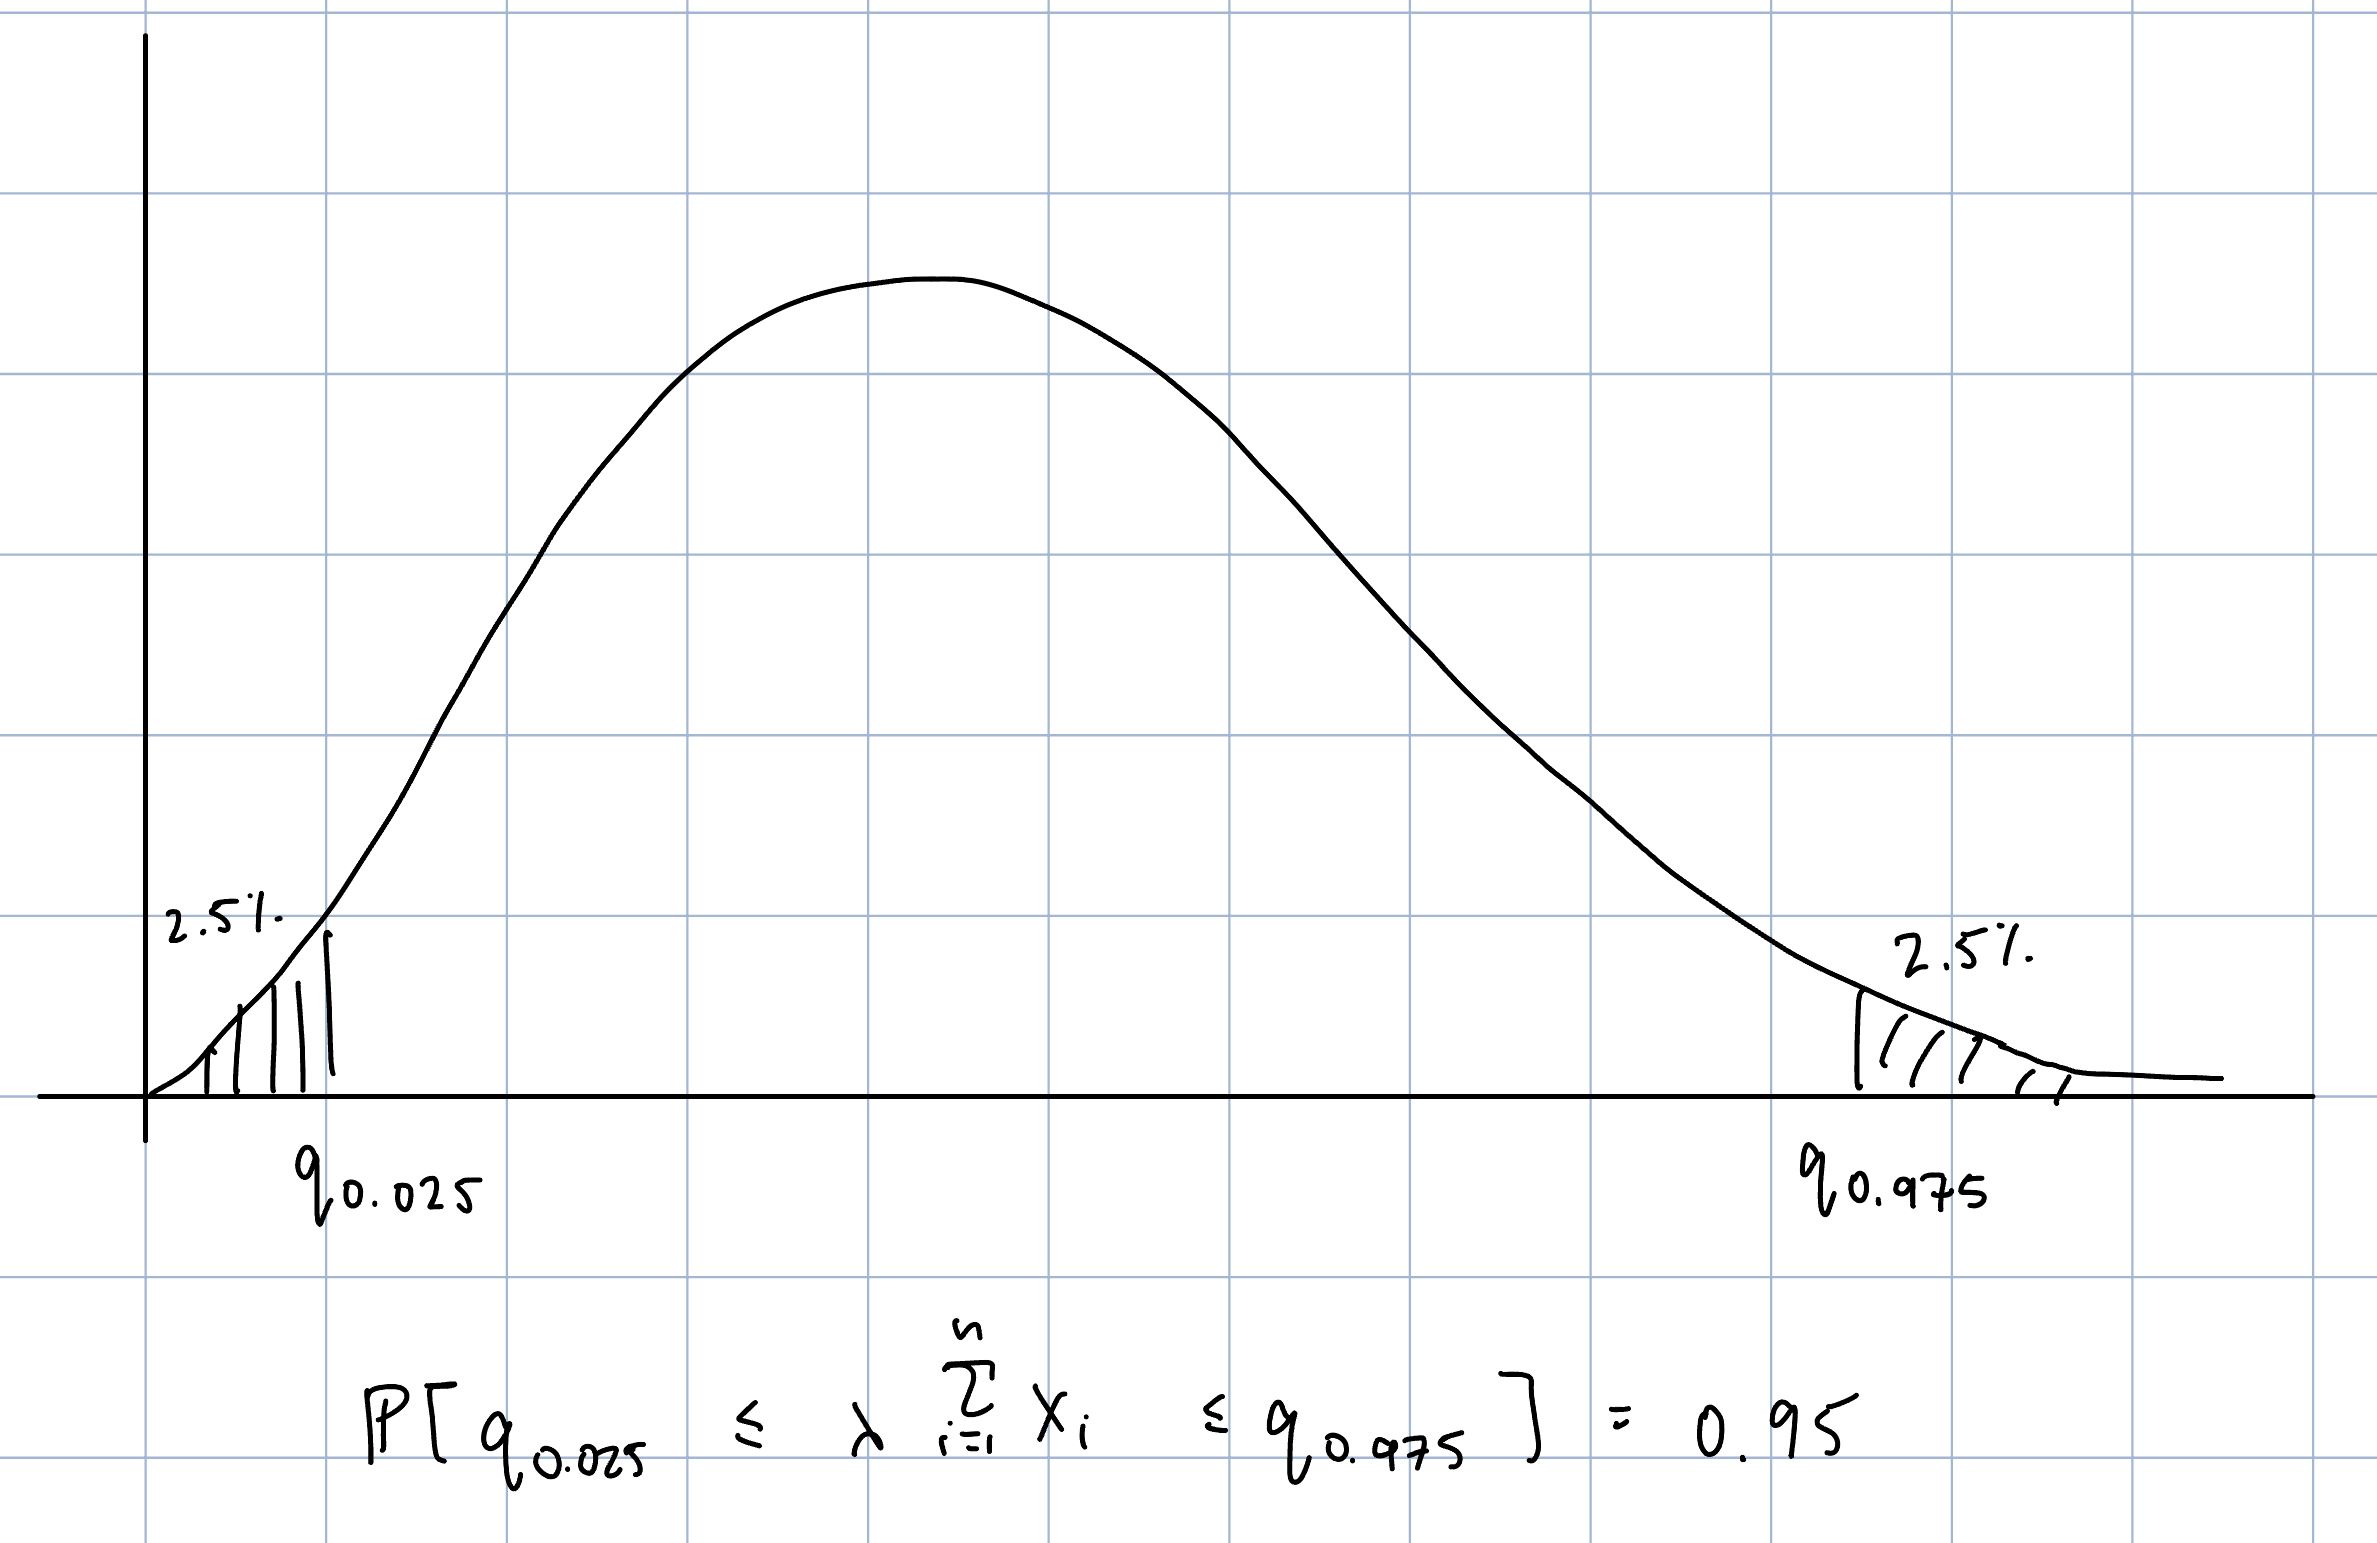
\includegraphics[width=0.9\textwidth]{10-30-1}
		\captionof{figure}{Density of $\lambda \sum\limits_{i=1}^{n} X_i$.}
	\end{center} \marginnote{Define quantiles as $q_\alpha$ satisfying $\P\left[Y \le q_\alpha\right] = \alpha$.}

	We see that \[
		\P\left[\frac{q_{0.025}}{\sum\limits_{i=1}^{n} X_i} \le \lambda \le \frac{q_{0.975}}{\sum\limits_{i=1}^{n} X_i}\right] = 0.95
	,\] so \[
		\left[ \frac{q_{0.025}}{\sum X_i}, \frac{q_{0.975}}{\sum X_i} \right] 
	\] is a 95\% confidence interval for $\lambda$.

	The key here is that we know the quantiles thanks to our realization that $\lambda \sum X_i \sim  \Gamma(n,1)$, which we know. $\lambda \sum X_i$ has a distribution that does not depend on $\lambda$.
	
\end{ex}

\begin{defn}[Pivot statistic]
	Suppose $X_1,\ldots,X_n$ are i.i.d. according to $F_\theta$. $g(X_1,\ldots,X_n,\theta)$ is called a pivot statistic if its distribution does not depend on $\theta$.
\end{defn}

\begin{rmk}
	If we have \[
		g(X_1,\ldots,X_n, \theta) \sim  F^*
	,\] where $F^*$ does not depend on $\theta$, we find the lower and upper quantiles $L,U$ such that \[
		\P\left[L < g(X_1,\ldots,X_n,\theta) < U\right] = \alpha
	\] and solve the equation for $\theta$; points in this set (hopefully an interval) satisfy the defining property of a confidence interval.
\end{rmk}

\begin{ex}
	Consider the following examples:
	\begin{enumerate}[(i)]
		\item Suppose $X_1,\ldots,X_n$ are i.i.d. $N(\mu,\sigma^2)$ and we want to find a confidence interval for $\mu$. We found earlier the pivot statistic that involves $\mu$ whose distribution does not depend on $\mu$: \[
			g(X_1,\ldots,X_n) = T = \sqrt{n} \frac{\overline{X}-\mu}{S}\sim t_{n-1}
		.\] Then our interval is \[
			\left[ \overline{X} - t_{n-1}^{\frac{\alpha}{2}} \frac{s}{\sqrt{n} }, \overline{X} + t_{n-1}^{\frac{\alpha}{2}} \frac{s}{\sqrt{n} } \right] 
		.\] 
		\item Suppose we have the same $X_1,\ldots,X_n$ that are i.i.d. according to $N(\mu,\sigma^2)$ and we want to find a confidence interval for the normal variance $\sigma^2$. Our pivot statistic is \[
			g(X_1,\ldots,X_n) = V = (n-1) \frac{S^2}{\sigma^2} \sim  \chi^2_{n-1}
		.\]
		\item Suppose we have $X_1,\ldots,X_n$ that are i.i.d. according to $F$ and we want a confidence interval for $\mu = \E\left[X_i\right] $. The Central Limit Theorem tells us that \[
			\frac{\overline{X}-\mu}{\frac{\sigma}{\sqrt{n} }} \to_{\mathscr{D}} N(0,1)
		.\] Then we can say for large enough $n$, \[
			\frac{\overline{X}-\mu}{\frac{\sigma}{\sqrt{n} }} \dot{\sim} N(0,1)
		.\] 

		If $\sigma$ is known, then an approximate $\alpha$-confidence interval is \[
			\left[ \overline{X} - z_{\frac{\alpha}{2}}\frac{\sigma}{\sqrt{n} }, \overline{X} + z_{\frac{\alpha}{2}} \frac{\sigma}{\sqrt{n} } \right] 
		.\] If $\sigma$ is not known, we use the sample standard deviation instead: \[
			\left[ \overline{X} - z_{\frac{\alpha}{2}}\frac{S}{\sqrt{n} }, \overline{X} + z_{\frac{\alpha}{2}} \frac{S}{\sqrt{n} } \right] 
		.\]
		\item Suppose we have $X_1,\ldots,X_n$ i.i.d. according to $F_\theta$ and want to find a confidence interval for the MLE $\hat{\theta}$. Assume that the necessary conditions for Cram\'er-Rao hold. We saw that \[
				\sqrt{n} \left( \hat{\theta}-\theta \right) \dot{\sim} N\left(0,\frac{1}{I(\theta)}\right)
		.\] The RHS depends on $\theta$, but we can use our best guess of $\hat{\theta}$ to create a double approximation of \[
			\sqrt{n} (\hat{\theta}-\theta) \dot{\sim} N\left(0, \frac{1}{I(\hat{\theta})}\right)
		.\] 
	\item Suppose $X_1,\ldots,X_n$ are i.i.d. according to $N(\mu_1,\sigma_1^2)$, $Y_1,\ldots,Y_n$ are i.i.d. according to $N(\mu_2,\sigma_2^2)$, and $(X_1,\ldots,X_n),(Y_1,\ldots,Y_n)$ are independent. If we want to find a confidence interval for $(\mu_1-\mu_2)$, we see \[
		\overline{X}-\overline{Y} \sim  N\left( \mu_1,\mu_2, \frac{\sigma_1^2}{n} + \frac{\sigma_2^2}{n} \right)
	,\] so we get \[
		\left( \overline{X}-\overline{Y} \right) - (\mu_1-\mu_2) \sim N\left(0, \frac{\sigma_1^2}{n} + \frac{\sigma_2^2}{n}
		\right).\] 
	\end{enumerate}
\end{ex}

\subsection{Bootstrap}

What if do not have a known distribution, as in the above cases? For instance, we might have $g \sim F^*$, where $F^*$ is unknown. We also might have an unbiased estimator $T_n$ of $\theta$ but not know $\operatorname{Var}(T_n)$.

\begin{defn}[Empirical distribution function]
	The EDF $\hat{F}_n$ of $X_1,\ldots,X_n$ i.i.d. according to $F$ is the cumulative density function that adds mass $\frac{1}{n}$ at each $X_i$. It has the form \[
		\hat{F}_n(x) = \frac{1}{n} \sum\limits_{i=1}^{n} \mathds{1}_{X_i \le x}
	.\] 
\end{defn}

\begin{rmk}
	We have the following properties of the EDF:
	\begin{enumerate}[(i)]
		\item For fixed $x$, $\hat{F}_n$ is a sample proportion for \[\operatorname{Bernoulli}(X_i \le x),\] which is just $\operatorname{Bernoulli}(F(x))$
		\item $\E\left[\hat{F}_n(x)\right] = F(x)$
		\item $\operatorname{Var}\left( \hat{F}_n(x) \right) = \frac{F(x) \left( 1-F(x) \right)}{n}$
		\item By the Law of Large Numbers, \[
			\hat{F}_n(x) \to_p F(x)
		.\] 
		\item (Glivenko-Cantelli Theorem) If $X_1,\ldots,X_n$ are i.i.d. according to $F$, \[
			\sup\limits_x \left| \hat{F}_n(x) - F(x) \right|\to 0
		.\] In other words, $\hat{F}_n \to F$ uniformly.
	\end{enumerate}
\end{rmk}

For the variable $\theta := T(F)$, we can construct the estimator $\hat{T} = T(\hat{F})$.

\begin{ex}
	For $T = \int_{}^{} x dF(x) $, $\theta$ is the mean. For $T = \int_{} (x-\mu)^2 dF(x) $, $\theta$ is the variance. For $T = F^{-1}(\frac{1}{2})$, $\theta$ is the median.
\end{ex}

\begin{ex} (Monte Carlo Simulation; Ideal Bootstrap)
	Let $X_1,\ldots,X_n$ be i.i.d. according to $F$ and let $T_n := g(X_1,\ldots,X_n)$. We want to find $\operatorname{Var}(T_n)$. If it is possible to sample from $F$, then we can repeat the following procedure:
	\begin{enumerate}[(i)]
		\item Take $k$ repeated samples of size $n$
		\item Calculate $T_n$ for each sample
	\end{enumerate}	
	to obtain $k$ samples $T_{n_1},\ldots,T_{n_k}$. We may use \[
		\frac{1}{k} \sum\limits_{i=1}^{k} \left( T_{n_i} - \overline{T}_n \right)^2
	\] as an estimator for $\operatorname{Var}\left(T_n\right)$.
\end{ex}

\begin{rmk}
	If we cannot directly sample from $F$, we may use $\hat{F}$ as an approximation. That is, given a sample of size $n$, we sample repeatedly with replacement $k$ samples also of size $n$ from the given sample, and calculate the statistic of interest for each sample to estimate the distribution of $T_n$. This procedure is called bootstrapping, and each sample is called a bootstrap sample.
\end{rmk}


\section{Hypothesis Testing}
\subsection{Basic Concepts}

Let $S_0$ denote the "acceptance" region and $S_1$ denote the rejection region of the parameter space $\Omega$ for the test statistic, so $S_0$ encodes outcomes in which we do not reject the null and vice versa. Let $\Omega_0$ be the null parameter space and $\Omega_1$ the alternative parameter space; i.e., where the null hypothesis is true and false. If we estimate the parameter well, then $S_i$ should coincide with $\Omega_i$. $\Omega = \Omega_1 \cup \Omega_2$ is the entire parameter space and $S = S_1\cup S_2$ is the entire data space.

\subsection{Type I and Type II Errors}


\begin{defn}[Power function]
	Let $X_1,\ldots,X_n$ be i.i.d according to $F_\theta$. The power function $\pi: \Omega\to [0,1]$ is such that \[
		\pi(\theta) = \P_\theta\left[ x \in S_1 \right] 
	.\] 
\end{defn}
\begin{rmk}
	From the power function, we can get the probability of type 1 and type 2 errors: the probability of a type 1 error is given by \[
		\pi(\theta), \quad \theta \in \Omega_0
	,\] while the probability of a type 2 error is given by \[
		1-\pi(\theta), \quad \theta \in \Omega_2
	.\] 
\end{rmk}

\begin{ex}
	Suppose $X_1,\ldots,X_n$ are i.i.d. according for $\operatorname{Unif}(0,\theta)$ for $\theta>0$. Our space is $\Omega = \R+$. Define \[
		H_0 : 3 \le \theta \le 4, \qquad
		H_A: \theta < 3 \text{ or } \theta > 4
		.\] Equivalently, \[
		\Omega_0 = [3,5], \qquad \Omega_1 = (0,3) \cup (5,\infty)
	.\] We know from before that the MLE of $\theta$ is the maximum of the sample observations, so the MLE is $X_{(n)} \in (0,\theta)$.

	The power function is \[
		\pi(\theta) = \P_\theta\left[ S_1 \right] = \P_\theta\left[ X_{(n)} \ge 4 \right] + \P_\theta\left[ X_{(n)} \le 2.99 \right] 
	.\]

	(Case 1: $\theta \le 2.99$) We have $\phi(\theta) = 0 + 1 = 1$.

	(Case 2: $2.99 < \theta < 4$) We have 
	\begin{align*}
		\pi(\theta) &= 0 + \P_\theta\left[ x_{(n)} \le 2.9 \right]  \\
					&= \left( \frac{2.99}{\theta} \right)^{n}
	.\end{align*}

	(Case 3: $\theta \ge 4$)\marginnote{I think the closed/openness of the boundaries of these regions is not quite right, but this is what was written down.} We have
	\begin{align*}
		\phi(\theta) &= \left[ 1-\P_\theta \left[ X_{(n)} < 4 \right]  \right] + \P_\theta\left[ X_{(n)} \le 2.9 \right] \\
					 &=1 - (\frac{4}{\theta})^{n} + \left( \frac{2.9}{\theta} \right)^{n}
	.\end{align*}
\end{ex}

Ideally, we would like \[ \begin{cases}
		0, \quad \theta \in \Omega_0 \\
		1, \quad \theta \in \Omega_1
	\end{cases}
,\] or just make $\pi$ low on $\Omega_0$ and high on $\Omega_1$.

\begin{defn}[Size of a test]
	Define the size of a test to be \[
		\sup\limits_{\theta \in \Omega_0} \pi(\theta)
	,\] which is the largest value of the power function when the true parameter lies in the null parameter region $\Omega_0$; it is a worst-case situation for trying to make $\pi$ low when the null hypothesis is actuall true.
\end{defn}

\begin{defn}[Level $\alpha$ test]
	A test is a level $\alpha$ test if the size of the test is less than $\alpha$; i.e., \[
		\sup_{\theta \in \Omega_0} \pi(\theta) \le \alpha
	.\] Note that as seen in our previous example, the size is usually difficult to evaluate. It is only easy to evaluate when $\Omega_0$ consists of a single point $\theta_0$.
\end{defn}

\begin{rmk}
	If $S_1 = \{T = T(X_1,\ldots,X_n\} \ge c$, then a level $\alpha$ test satisfies \[
		\sup_{\theta \in \Omega_0} \P_\theta\left[T \ge c\right] \le \alpha
	.\] 
\end{rmk}

\subsection{Examples of Tests}

\begin{ex}
	Suppose $X_1,\ldots,X_n$ are i.i.d. according to $F_\mu$, where $\E\left[X_i\right] =\mu$ is unknown and $\operatorname{Var}(X_i) = \sigma^2$ is known. Our hypotheses are \[
		H_0: \mu = \mu_0, \qquad H_A: \mu > \mu_0
	.\]  By the Central Limit Theorem, we know that $\sqrt{n} \frac{\overline{X}_n - \mu_0}{\sigma} \sim N(0,1)$, so we define our test statistic rejection region by putting $T = \sqrt{n} \frac{\overline{X}_n-\mu_0}{\sigma}$ and \[
		S_1 = \{T \ge c\}
	.\] We know that \[
		\P_{\mu_0}\left[x \in S_1\right] = \P_{\mu_1}\left[T \ge c\right] 
	.\] So we can set $c = z_\alpha$\marginnote{$z_\alpha$ is defined to be the quantile satisfying \[
		\P\left[z > z_\alpha\right] = \alpha
	\] for $z \sim  N(0,1)$ }

	The rejection region is \[
		\{x, \overline{X}_n \ge \mu_0 + z_\alpha \frac{\sigma}{\sqrt{n} }\}
	.\] 
\end{ex}

\begin{ex}
	Suppose $X_1,\ldots,X_n$ are i.i.d. according to $F_\mu$, where $\E\left[X_i\right] =\mu$ is unknown and $\operatorname{Var}(X_i) = \sigma^2$ is known. Our hypotheses are \[
		H_0: \mu = \mu_0, \qquad H_A: \mu \ne \mu_0
	.\] Then the rejection region is \[
		S_1 = \{\left| T \right| \ge c_1\}
	.\] We get \[
		\P_{\mu_0}\left[S_1\right] = \alpha \implies \qquad c_1 = z_{\frac{\alpha}{2}}
	.\] Then \[
		S_1 = \{\left| T \right|\ge z_{\frac{\alpha}{2}}\}
	.\] 

	What is the power of this test?
	\begin{align*}
		\pi(\mu) = \P_\mu\left[S_1\right] &= \P_\mu\left[\left| \sqrt{n} \frac{\overline{X}_n-\mu_0}{\sigma} \right| \ge z_{\frac{\alpha}{2}}\right]  \\
										  &= \P_\mu\left[\sqrt{n} \left| \frac{\overline{X}_n-\mu}{\sigma}+\frac{\mu-\mu_{0}}{\sigma} \right| \ge z_{\frac{\alpha}{2}}\right] \\
										  &= \P\left[\sqrt{n} \left| z + \frac{\mu-\mu_0}{\sigma} \right|\ge z_{\frac{\alpha}{2}}\right]  \\
										  &= \P\left[\sqrt{n} \left( z+ \frac{\mu-\mu_0}{\sigma} \right) \ge z_{\frac{\alpha}{2}}\right] + \P\left[\sqrt{n} \left( z + \frac{\mu-\mu_0}{\sigma} \right) \le -z_{\frac{\alpha}{2}}\right] \\
										  &= \P\left[z \ge \frac{1}{\sqrt{n} }\left( z_{\frac{\alpha}{2}} - \frac{\mu-\mu_0}{\sigma} \right)\right] + \P\left[z \le \frac{1}{\sqrt{n} }\left( -z_{\frac{\alpha}{2}} - \frac{\mu-\mu_0}{\sigma} \right)\right]  
	.\end{align*}
	The power depends on the sample size $n$ and the signal $\mu-\mu_0$.
\end{ex}

\begin{ex}
	Suppose $X_1,\ldots,X_n$ are i.i.d. according to $F_\mu$, where $\E\left[X_i\right] =\mu$ is unknown and $Var(X_i) = \sigma^2$ is also unknown. Then \[
	T = \sqrt{n} \frac{\overline{X}_n-\mu_0}{S} \approx t_{n-1}
	.\] 
\end{ex}

\begin{ex}
	(Variance of Normal) Suppose $X_1,\ldots,X_n$ are i.i.d according to $N(\mu,\sigma^2)$. Let \[
		H_0: \sigma = \sigma_0, \qquad H_A: \sigma \ne \sigma_0
	.\]  We have \[
		\Omega_0 = \R \times \{\sigma_0\}, \qquad \Omega_1 =\R\times \R\setminus \{\sigma_0\}
	.\] 
	We use \[
		T = (n-1) \frac{S^2}{\sigma_0^2} \underbrace{\sim \chi_{n-1}^2}_{\text{under } H_0}
	.\] Intuitively, we reject when $T$ is small and when $T$ is large; \[
		S_1 = \{T < L, T > U\}
	\] for $L,U$ we need to select.
	
	We want $L,U$ to satisfy \[
		\P_{\sigma_0}\left[S_1\right] = \alpha
	.\] $L,U$ should be quantiles of $\chi_{n-1}^2$ that satisfy this.\marginnote{But then $L,U$ aren't unique since $\chi^2$ is not symmetric?}

	Writing \[
		T = (n-1) \frac{S^2}{\sigma_0^2} = (n-1) \frac{S^2}{\sigma^2} \frac{\sigma^2}{\sigma_0^2}
	,\] the power is
	\begin{align*}
		\P_\sigma\left[S_1 \right] &= \P_\sigma\left[T > L, T > U\right] \\
		&= \P\left[\chi_{n-1}^2 < L \frac{\sigma_0^2}{\sigma^2}, \chi_{n-1}^2 > U \frac{\sigma_0^2}{\sigma^2}\right] 
	.\end{align*}
\end{ex}

\subsection{p-values}
\begin{defn}[p-value]
	The p-value is the smallest level $\alpha$ for which we reject the null with the observed data.
\end{defn}
\begin{rmk}
	If we calculate the p-value, we do not need to specify $\alpha$, as if $\alpha$ is larger than the p-value, we reject the null, and if $\alpha$ is less than the p-value, we do not reject the null.
\end{rmk}

\begin{ex}
	Suppose $X_1,\ldots,X_n$ are i.i.d. according to $F$, where $\E\left[X\right] = \mu$ is unknown and $\operatorname{Var}\left(X\right) = \sigma^2$ is known.
	Put \[
		H_0: \mu = \mu_0, \qquad H_A: \mu > \mu_0
	.\] Then our test statistic is \[
		T(X) = \sqrt{n} \frac{\overline{X}_n - \mu_0}{\sigma} \sim N(0,1), \quad \text{if $H_0$ is true}
	.\] We decided previously that the rejection region is $\{T(X) \ge z_\alpha\}$.

	Given some realized data $X_1,\ldots,X_n$ and the corresponding test statistic $T_{obs}$, then the p-value is the $\alpha'$ for which equality holds: \[
		T_{obs}(X) = z_{\alpha'}
	.\] Alternatively, if $z \sim  N(0,1)$, then the p-value $\alpha'$ is \[
		\alpha' = \P\left[z \ge T_{obs}\right] 
	.\] 
\end{ex}
\begin{ex}
	Consider the same environment but the new hypotheses: \[
		H_0: \mu = \mu_0, \qquad H_a: \mu \ne \mu_0
	.\] 
	Then our rejection region is \[
		S_1 = \{\left| T(x) \right| > z_{\frac{\alpha}{2}}\}
	.\] The p-value is $\alpha'$ such that \[
		\P\left[z \ge \left| T \right|\right] = \frac{\alpha}{2}
	,\] or \[
		\alpha' = 2\P\left[z \ge \left| T \right|\right] 
	.\] 
\end{ex}

\begin{rmk}
	If $\Phi$ is the CDF of the standard normal distribution, then \[
		\text{p-value} = \P\left[z \ge T_{obs}\right] = 1 - \P\left[z < T_{obs}\right] = 1- \Phi(T)
	\] is $\operatorname{Unif}(0,1)$ under the null hypothesis.
	This helps us in the interpretation of p-values.
\end{rmk}

\begin{ex}
	(Comparing variances) Consider $X_1,\ldots,X_n$ i.i.d. from $N(\mu_1,\sigma_1^2)$ and $Y_1,\ldots,Y_n$ from $N(\mu_2,\sigma_2^2)$. Put \[
		H_0: \sigma_1^2 = \sigma_2^2, \qquad H_A: \sigma_1^2 \ne \sigma_2^2
	.\]\marginnote{Note that $\Omega_0 = \{(\mu,\sigma_1,\mu_2,\sigma_2) \in \R^{4} : \sigma_1^2=\sigma_2^2\}$. Since $\Omega_0$ is so complicated, we want one has the same distribution on all these \texthl{(?)} values.}

	Recall that \[
		\frac{(n-1)S_X^2}{\sigma_1^2}\sim \chi_{n-1}^2, \qquad \frac{(n-1)S_Y^2}{\sigma_2^2} \sim  \chi_{n-1}^2
	.\] 
	Further note that \[
		U \sim \chi_m^2, \quad V \sim \chi_n^2 \implies \frac{\frac{U}{m}}{\frac{V}{n}} \sim  F_{m,n}
	,\] where $F$ does not depend on $\sigma_1, \sigma_2$. This implies that \[
		\frac{\frac{S_X^2}{\sigma_1^2}}{\frac{S_Y^2}{\sigma_2^2}} \sim  F_{m-1, n-1}
	.\] 
	Our test statistic is \[
		T(X,Y) = \frac{S_X^2}{S_Y^2} \sim_{H_0} F_{n-1,m-1}
	.\] Because we have a two-sided test, our rejection region is \[
		S_1 = \{T > U\} \cup \{T < L\}
	.\] 

\end{ex}

\subsection{Likelihood Ratio Tests}
We wonder how we can systematically come up with test statistics. Suppose $X_1,\ldots,X_n$ are i.i.d. according to $F_\theta$ that has density $f(x\mid \theta)$. 

We start with simple point hypotheses: consider \[
	H_0: \theta = \theta_0, \qquad H_A: \theta - \theta_1
.\] The likelihood ratio is defined \[
	LR(X) = \frac{L(\theta_0 \mid X)}{L(\theta_1 \mid X)} = \frac{\prod_{i=1}^{n} f(X_i \mid \theta_0) }{\prod_{i=1}^{n} f(X_i \mid \theta_1) }
.\] We want to reject the null when $L(\theta_1 \mid X)$ is much larger than $L(\theta_0 \mid X)$, so the rejection region looks like \[
	S_1 = \{LR \le c\}
\] for $c \in \R$.

\begin{ex}
	Consider \[
		H_0: X_1,\ldots,X_n \text{ i.i.d. according to } N(1,1), \qquad H_A: X_1,\ldots,X_n \text{ i.i.d. according to } N(2,2)
	.\] 
	In this case, we have $\theta = (\mu,\sigma^2)$.
	The likelihood ratio is 
	\begin{align*}
		LR(X) &= \frac{\left( \frac{1}{\sqrt{2\pi} } \right)^{n} \exp{\left(-\sum\limits_{i=1}^{n} \frac{\left( X_i -1 \right)^2}{2}\right)}}{\left( \frac{1}{\sqrt{2} \sqrt{2\pi} } \right)^{n} \exp{\left(-\sum\limits_{i=1}^{n} \frac{\left( X_i - 2 \right)^2}{2\cdot 2}\right)}} \\
		&= \left( \sqrt{2}  \right)^{n} \exp{\left(-\sum\limits_{i=1}^{n} \left[ \frac{X_i^2}{2}-X_i + \frac{1}{2} - \frac{X_i^2}{4} + X_i - 1 \right]\right)} \\
		&= \left( \sqrt{2}  \right)^{n} e^{\frac{n}{2}} \exp\left(- \sum\limits_{i=1}^{n} \frac{X_i^2}{4} \right)
	.\end{align*}
	If you think enough, the test statistic makes sense.
	The rejection region is \[
		S_1 = \{\sum X_i^2 \ge c\}
	.\] 
\end{ex}

\begin{prop}
	(Neyman-Pearson Lemma) \marginnote{Setting this up with simple hypotheses does not seem very useful. This fact motivates the General Likelihood Ratio Test.}For simple hypotheses $H_0,H_A$, if we define \[
		S_1 = \{LR \le c\}, \quad \alpha = \P\left[\text{type I error}\right], \quad \beta = \P\left[\text{type II error}\right] 
	,\]  then any other test with the same $\alpha$ as the likelihood ratio test has a larger $\beta$.

	In other words, fixing a type 1 error rate, any other test has a larger type 2 error compared to the Likelihood Ratio test; the LR test is optimal in this sense.
\end{prop}

\begin{proof}
	We skip the proof.
\end{proof}

\begin{defn}[General Likelihood Ratio Test]
	Consider the general situation \[
		H_0: \theta \in \Omega_0, \qquad H_A: \theta \in \Omega_1, \quad \Omega_0 \cup \Omega_1 = \Omega
	.\] Put \[
		\Lambda(X) = \frac{\sup_{\theta \in \Omega_0} L\left(\theta \mid X) \right)}{\sup_{\theta \in \Omega_1} L(\theta \mid X)}
	.\] 
\end{defn}

\begin{thm}
	\marginnote{Once we show this, we will have an automatic test statistic for hypothesis tests.}Let $\Omega \subset \R^p$ be open and suppose $\Omega_0$ is obtained by fixing $k$ coordinates. If the MLE assumptions are satisfied, \[
		-2 \ln{\left(\Lambda(X)\right)} \sim_{H_0} \chi_k^2
	.\] 
\end{thm}

\begin{ex}
	Suppose $X_1,\ldots,X_n$ is i.i.d. according to $N(\mu,\sigma^2)$. In this case, $p = 2$. With the null hypothesis \[
		H_0: \mu = \mu_0
	,\] we have $k=1$ since only one coordinate of the parameter space $\Omega$ is fixed. Instead, if \[
		H_0: \mu=0, \sigma^2 = 1
	,\] then $k=2$.
\end{ex}

\begin{proof}
	(Case 1) Consider $\theta \in \Omega \subset \R$ with \[
		H_0: \theta = \theta_0
	.\] Then $p = k = 1$, so we want to show that $-2\ln{\left(\Lambda(X)\right)}\sim \chi^2_1$ under the null.

	Let $\hat{\theta}$ be the MLE. Then we can Taylor expand the log-likelihood to see
	\begin{align*}
		-2 \ln{\left(\Lambda(X)\right)} &= -2\left( l(\theta_0) - l(\hat{\theta}) \right) \\
		l(\theta_0) &\approx l(\hat{\theta}) + (\theta_0-\hat{\theta})\dot{l}(\hat{\theta}) + \frac{1}{2} (\theta_0-\hat{\theta})\ddot{l}(\hat{\theta}) \\
		\implies -2 \left( l(\theta_0) -l(\hat{\theta}) \right) &\approx \left( \hat{\theta}-\theta_0 \right)^2 \left[ -\ddot{l}(\hat{\theta}) \right]
	.\end{align*}
	The first term in the product is the normal square, and the second is the Fisher information of $\theta_0$.
\end{proof}

\subsection{Relating Hypothesis Testing and Confidence Intervals}
\begin{ex}
	Let $X_1,\ldots,X_n$ be i.i.d\ according to $N(\mu,1)$. We are interested in \[
		H_0: \mu = \mu_0, \qquad H_A: \mu \ne 0
	.\] We used the test statistic \[
		T = \sqrt{n}  \left| \frac{\overline{X}_n - \mu_0}{1} \right|
	\] to find the acceptance and rejection regions at level $\alpha$ \[
		S_0 = \left\{x: \mu_0 - \frac{z_{\frac{\alpha}{2}}}{\sqrt{n} } \le \overline{X} \le \mu_0 + \frac{z_{\frac{\alpha}{2}}}{\sqrt{n} }\right\}, \quad S_1 = \{x: \sqrt{n} \left| \overline{X} - \mu_0 \right| > z_{\frac{\alpha}{2}}\}
	.\] Note that $S_0 = \left\{x: \overline{X}_n - \frac{z_{\frac{\alpha}{2}}}{\sqrt{n} } \le \mu_0 \le \overline{X}_n + \frac{z_{\frac{\alpha}{2}}}{\sqrt{n} }\right\}$, which we read as: ``Given the data $X_1,\ldots,X_n$, any $\mu_0$ such that $\mu \in \left[ \overline{X}_n - \frac{z_{\frac{\alpha}{2}}}{\sqrt{n} }, \overline{X}_n + \frac{z_{\frac{\alpha}{2}}}{\sqrt{n} } \right]$ is not rejected by the test.

	Note that $\left[  \overline{X}_n - \frac{z_{\frac{\alpha}{2}}}{\sqrt{n} }, \overline{X}_n + \frac{z_{\frac{\alpha}{2}}}{\sqrt{n} } \right]$ is an $(1-\alpha)$-confidence interval! 
\end{ex}

\begin{prop}
	In the general case, suppose $X_1,\ldots,X_n$ are i.i.d.\ according to $F_\theta$ and let $A(\theta_0)$ be the acceptance region at level $\alpha$ of \[
		H_0 : \theta = \theta_0, \qquad H_A: \theta \ne \theta_0
	.\] Let \[
		S(x) = \{\theta_0 : x \in A(\theta_0)\}
	,\] which is the set of all parameters $\theta_0$ for which the null is accepted (not rejected) by the data. We have that $S(x)$ is a $(1-\alpha)$-confidence set.
\end{prop}
\begin{proof}
	Note that 
	\begin{align*}
		\P_\theta\left[\theta \in S(x)\right] &= \P_\theta\left[x \in A(\theta)\right] \\
											  &\ge 1-\alpha
	.\end{align*}
\end{proof}
\begin{rmk}
	Note that the reverse is true; we can start with a confidence set and construct a dual hypothesis test.

	Let $S(x)$ be a ($1-\alpha$)-confidence set and $A(\theta) = \{x: \theta_0 \in S(x)\}$. Then $A(\theta_0)$ is the acceptance region for a level-$\alpha$ test of \[
		H_0: \theta = \theta_0
	.\] 
\end{rmk}

\subsection{Multiple Hypothesis Testing}

Recall the example from the very first lecture this quarter:
\begin{ex}
	In a genome-wide association study, we might have 1 million single nucleotide polymorphisms, so we have 1 million tests and 1 million p-values. Under the null, the p-values are approximately distributed according to $\operatorname{Unif}(0,1)$, so we expect many p-values to be very low.
\end{ex}

Suppose we have $m$ tests and $p_1,\ldots,p_m$ are their p-values. For simplicity, assume that the p-values are independent.\marginnote{This independence assumption does not hold up in the GWAS context.} If all the null hypotheses are true, then \begin{align*}
	\P\left[\text{at least one p-value } \le \gamma\right] &= \P\left[p_{(1)} \le \gamma\right] \\ 
														   &= 1 - \P\left[p_{(1)} > \gamma\right] \\ 
														   &= 1 - (1-\gamma)^{m}
.\end{align*}
For $m=1000$ and $\gamma=0.001$, the probability is $0.62$. 

What is the level of $\gamma$ necessary to control the probability of a type I error? We want
\begin{align*}
	1-\left( 1-\gamma \right)^{m} &\le \alpha \\
	(1-\alpha)^{\frac{1}{m}} &\le 1- \gamma \\
	\gamma &\le 1 - \left( 1-\alpha \right)^{\frac{1}{m}}
.\end{align*}

\begin{rmk}
	We know that $e^x \approx 1+x$ for small $x$. So 
	\begin{align*}
		1-(1-\alpha)^{\frac{1}{m}} &\approx 1- e^{-\frac{\alpha}{m}} \\
								   &\approx 1- (1-\frac{\alpha}{m}) \\
								   &= \frac{\alpha}{m}
	.\end{align*}
	So the control necessary is roughly \[
		\gamma < \frac{\alpha}{m}
	,\] the Bonferroni correction. 
\end{rmk}

\marginnote{
	\begin{center}
		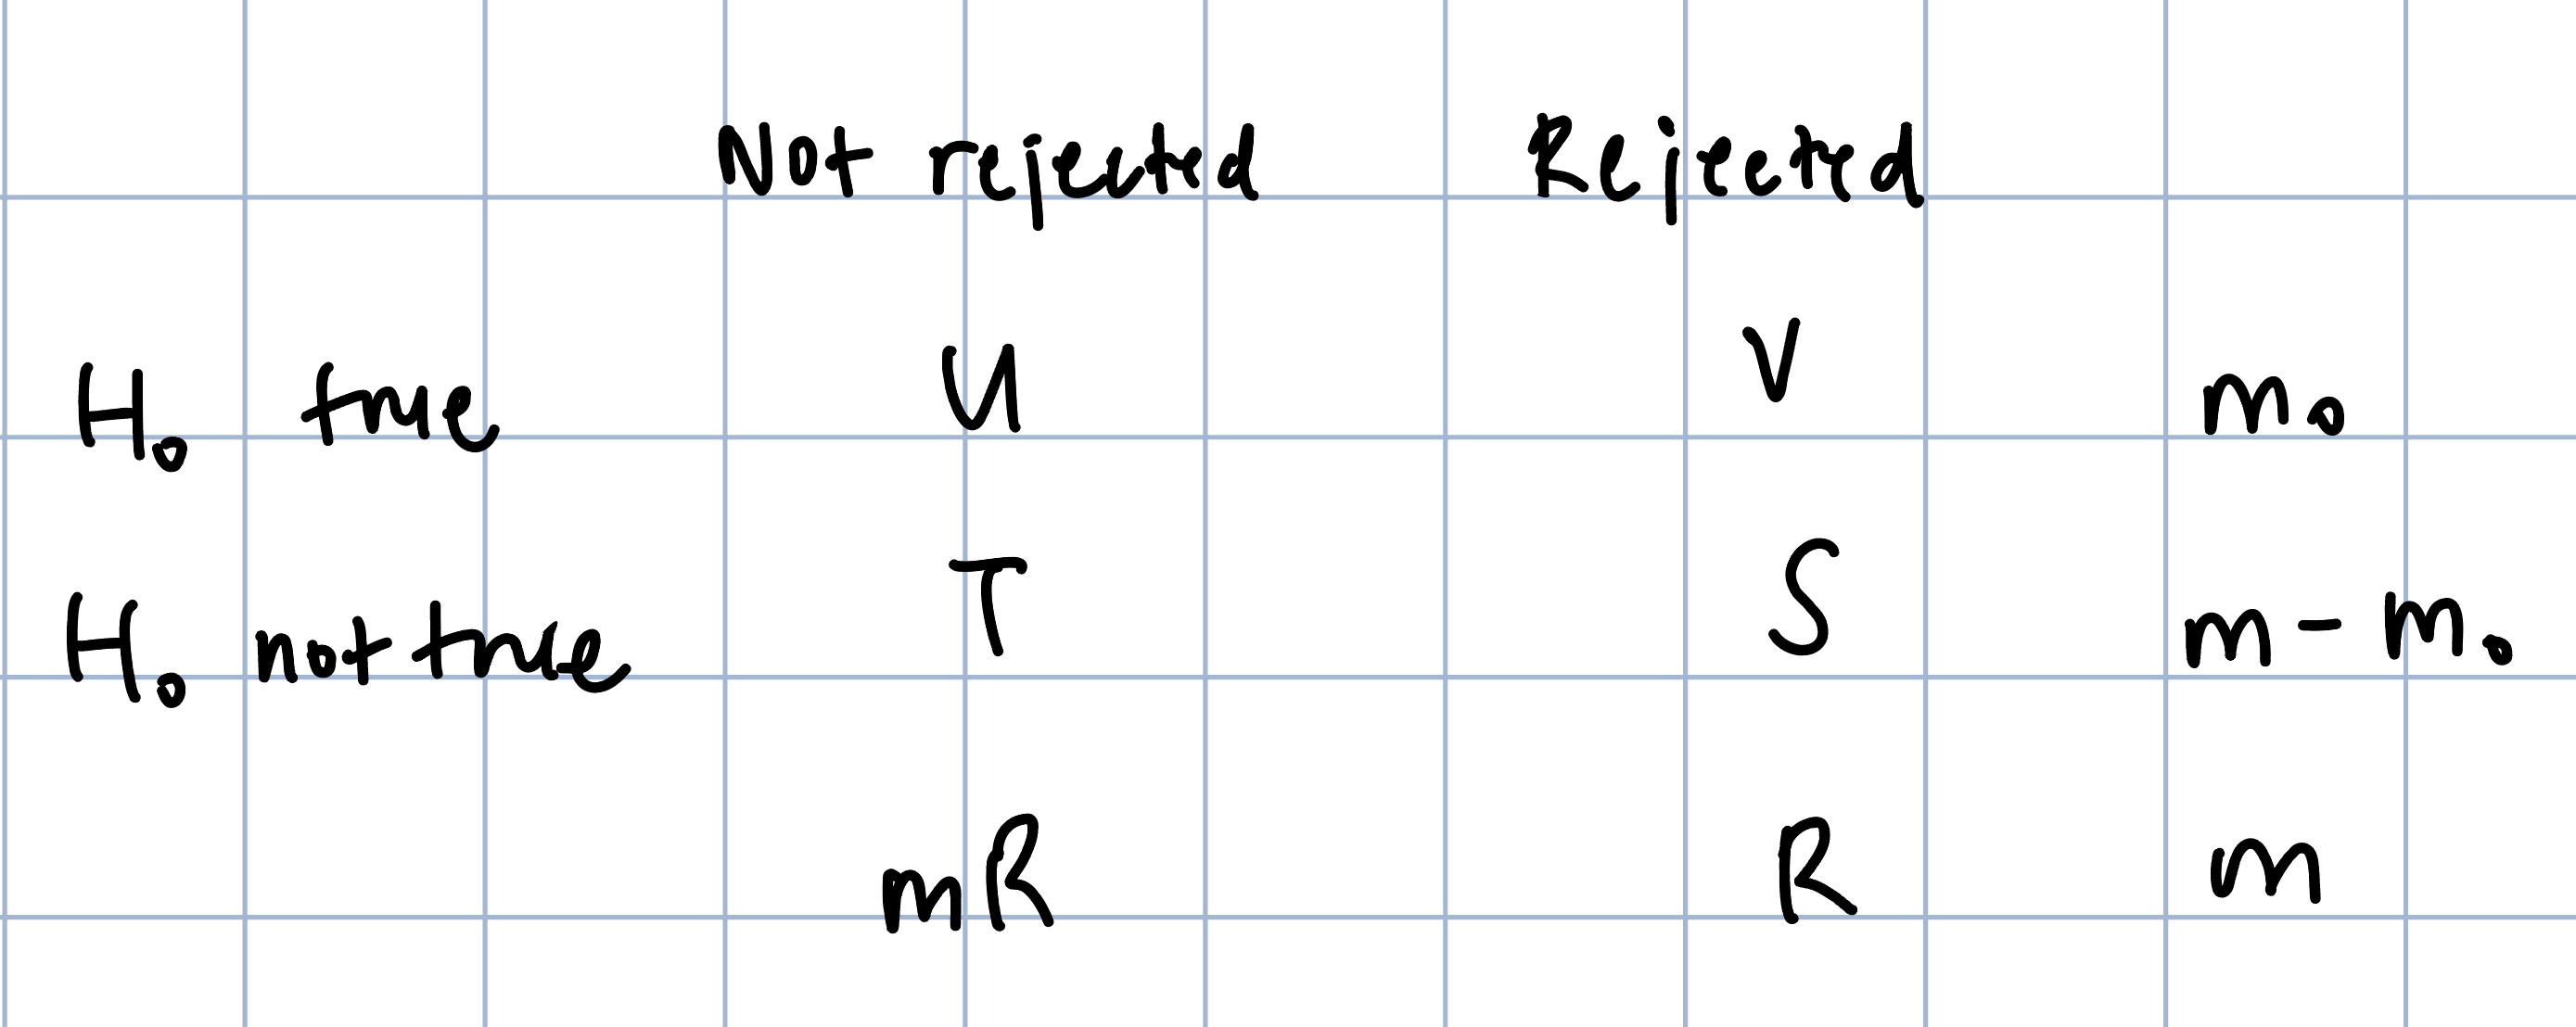
\includegraphics[width=0.5\textwidth]{11-18-1}
		\captionof{figure}{Counts in Multiple Hypothesis Testing}
	\end{center}
}
Referring to the table on the right, $V$ is the number of false positives and $T$ is the number of false negatives. 

\begin{defn}[Family-wide error rate]
	Define the FWER as $\P\left[V > 0\right] $, 
\end{defn}
\begin{ex}
	In the GWAS context, if $m=10^{6}$ and $\alpha = 0.05$, then we require \[
		\gamma < \frac{\alpha}{m} = 5 \cdot 10^{-8}
	.\] 
	This number is so low because we required that there were exactly 0 false positives.
	What is more common is allowing for some number of false positives then repeat the experiment in a new context (for example, a new population)
\end{ex}

The extremely low requirements for p-values under Bonferroni correction motivates the following statistics.

\begin{defn}[Per-family error rate]
	Define the PFER as $E(V)$.
\end{defn}

\begin{defn}[False Discovery Rate (FDR)]
	Define the FDR as $\E\left[\frac{V}{R}\right] $.
\end{defn}

\begin{thm}
	(Benjamini \& Hochberg)\marginnote{This comes from the widely-cited 1995 paper from the authors who name the result after themselves.} 
	Suppose we want to control the FDR at level $\alpha$. Order the p-values $p_{(1)} \le \ldots \le p_{(m)}$. Find the largest $j$ such that $p_{(j)} \le \frac{\alpha j}{m}$. Reject all hypotheses corresponding to \[
		p_{(1)},\ldots,p_{(j)}
	.\] 
\end{thm}
Given a rejection region $[0,\gamma]$, we see that $\E\left[V\right]  = m_0 \gamma$. We need to know $m_0$ or \[
	\pi_0 = \frac{m_0}{m}
.\]
\marginnote{
	\begin{center}
		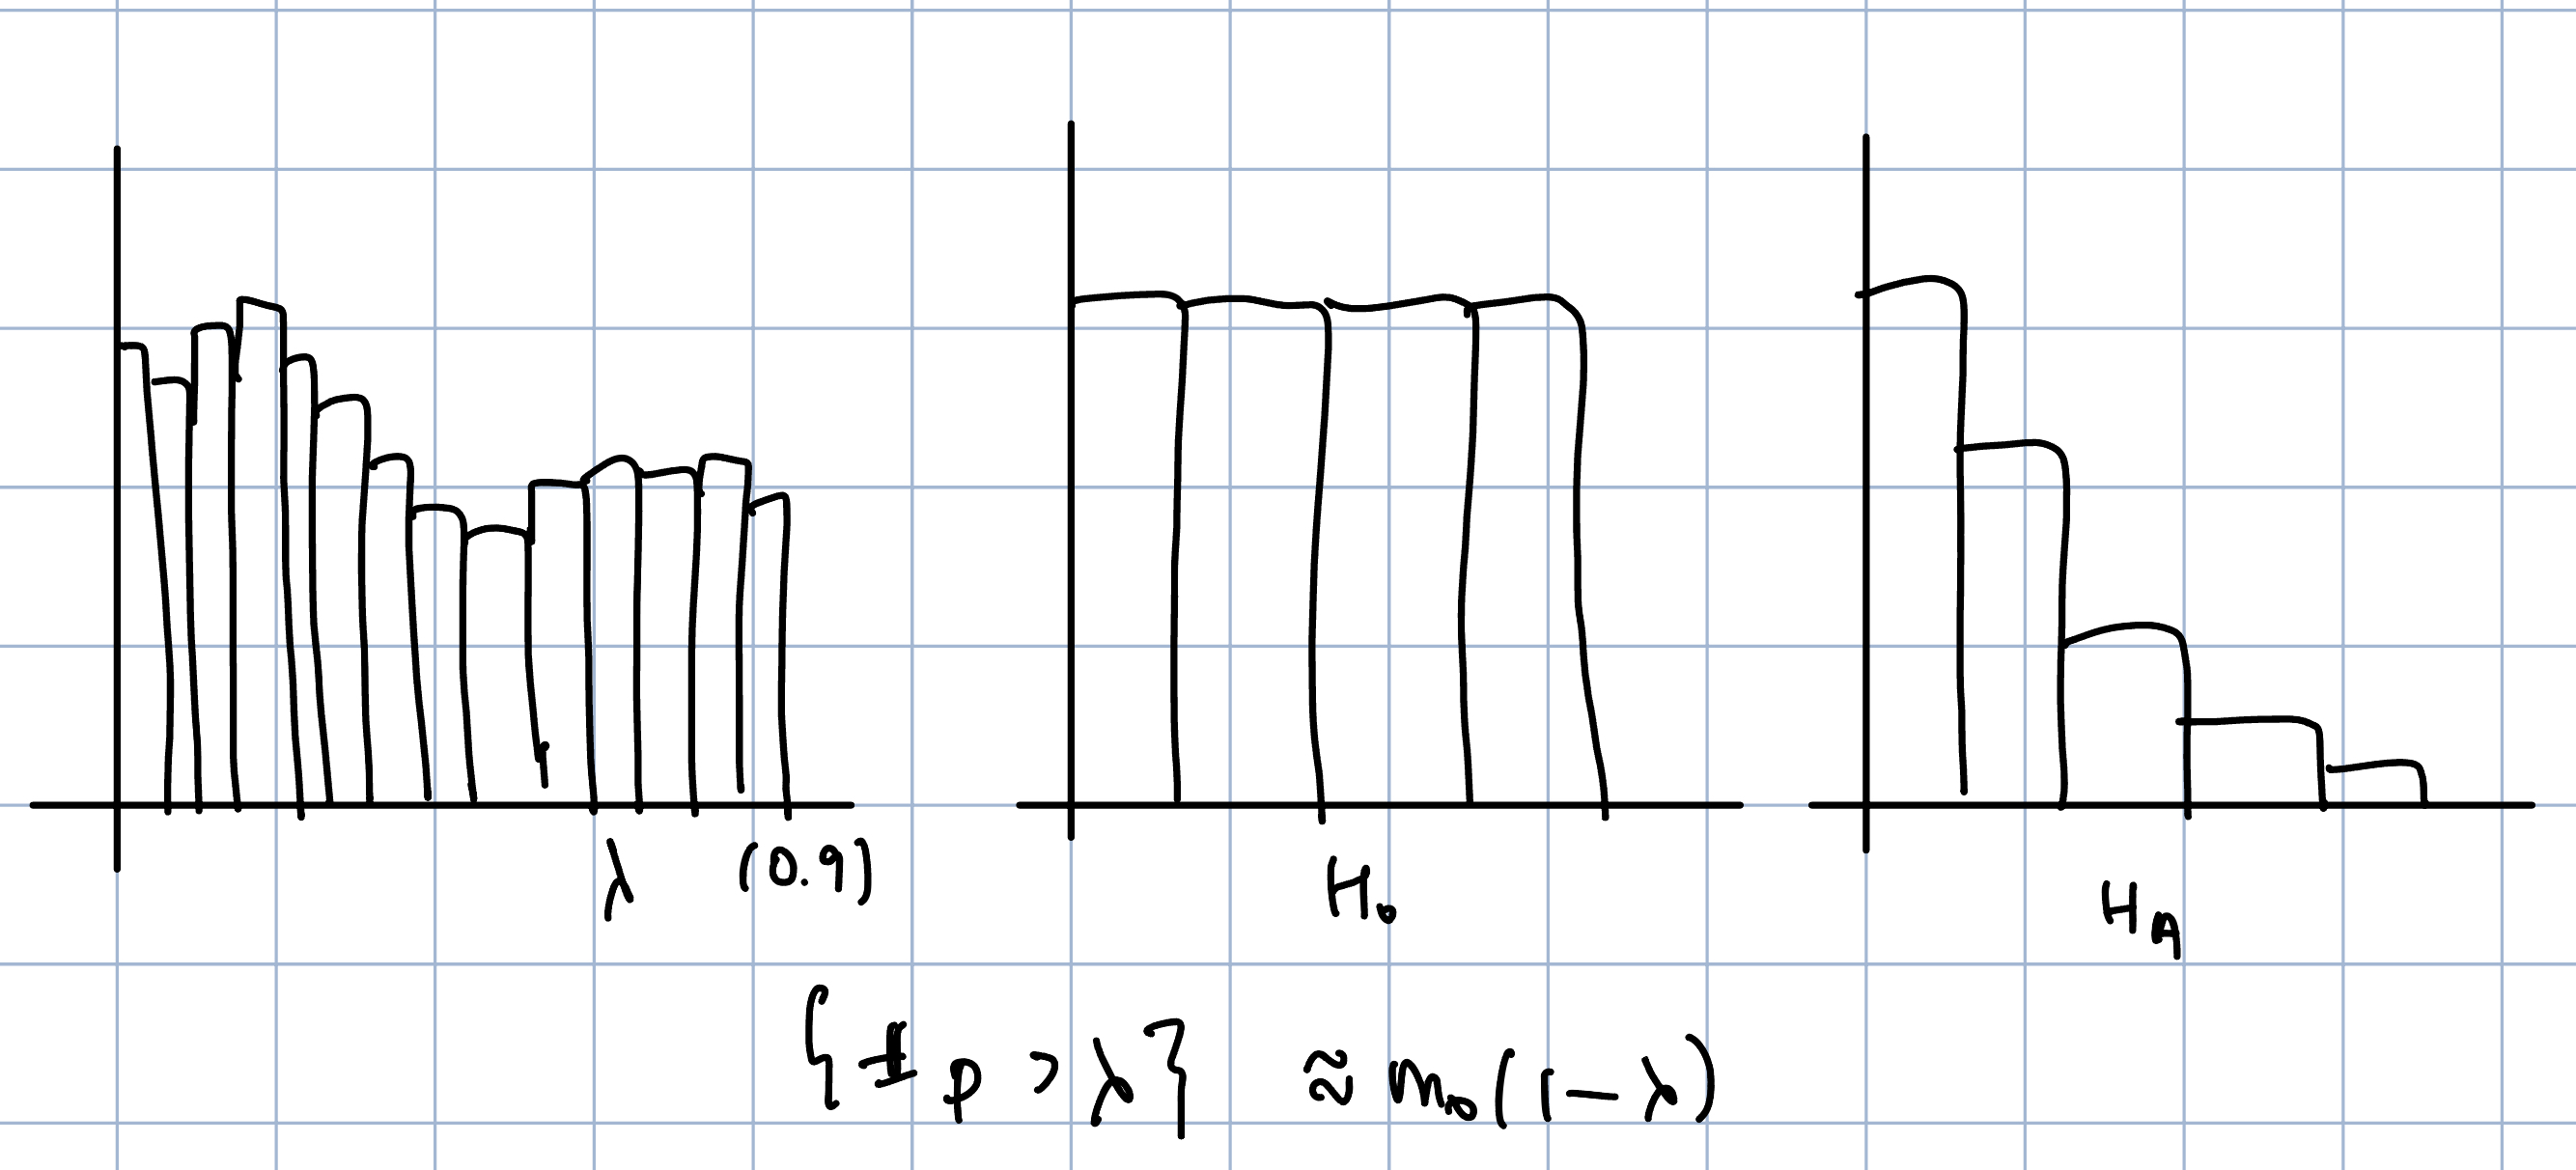
\includegraphics[width=0.5\textwidth]{11-18-2}
		\captionof{figure}{Histograms of all p-values under $H_0$ and $H_A$.}
	\end{center}
}
Referring to the histograms, we see that \[
	FDR \approx \frac{m_0 \gamma}{R} = \frac{\{p > \lambda\} \gamma}{(1-\lambda)R}
.\] When $\lambda = 0.99$, you know that most most of the p-values will be coming from the null (?). But a large $\lambda$ means that you have a low sample size --- we see the same tradeoff where the bias is small but variance is large.

\begin{proof}
	(Benjamini \& Hochberg) Define $\alpha_r = \frac{\alpha r}{m}$ for $r = 1,\ldots,m$. Then\marginnote{$\alpha_R$ is the threshold for having $R$ discoveries (total number of tests rejected)} \begin{align*}
		\E\left[\frac{V}{R}\right] &= \E\left[\frac{\sum\limits_{k \in \N}^{} \mathds{1}_{\{p_k \le \alpha_R\}}}{R}\right] \\
								   &= \sum\limits_{k\in \N}^{} \sum\limits_{n=1}^{m} \frac{1}{r}\P\left[p_k \le \alpha_R ,R = r\right] 
							   .\end{align*}
	The trick is to let $R_k$ be the number of discoveries when doing Benjamini-Hochberg at level $\alpha$ with $p_k$ replaced by $0$.
	As a result,
	\begin{align*}
		\P\left[p_k \le \alpha_R, R = r\right] &= \P\left[p_k \le \alpha_r, R_k = r\right]  \\
		&= \P\left[p_k \le \alpha_r\right] \P\left[R_k = r\right]
	,\end{align*} so 
	\begin{align*}
		\E\left[\frac{V}{R}\right] &= \sum\limits_{k\in N}^{} \sum\limits_{r=1}^{n} \frac{1}{r \alpha_R \P\left[R_k = r\right] }\\
								   &= \sum\limits_{k\in N}^{} \frac{\alpha}{m} \sum\limits_{i=1}^{n} \P\left[R_k = r\right] \\
								   &= \sum\limits_{k \in N}^{} \frac{\alpha}{m} \\
								   &= \alpha \frac{m_0}{m}
	.\end{align*}
\end{proof}

\section{Bayesian Statistics}
\subsection{Bayes' Formula}

\begin{defn}[Bayes' formula]
	Bayes' formula is given by \[
		\P\left[A \mid B\right] = \frac{\P\left[B \mid A\right] \P\left[A\right] }{\P\left[B\right] }
	.\] 	
\end{defn}

Suppose $H_1,\ldots,H_k$ is a partition of the sample space $S$ and $D$ is an event such that $\P\left[D\right] > 0$. Then as a result of Bayes' formula, we have \[
	\P\left[H_i \mid D\right] = \frac{\P\left[H_i\right] \P\left[D \mid H_i\right] }{\sum\limits_{i=1}^{k} \P\left[H_j\right] \P\left[D \mid H_j\right] }
,\] where the denominator comes from the Law of Total Probability. This expression represents how beliefs are updated in light of new information.

\begin{ex}
	Consider people who have some combination of coronary artery disease and peripheral artery disease. We can partition the sample space into \begin{align*}
		&H_1 = \{CAD^+, PAD^+\}, \quad H_2 = \{CAD^+, PAD^-\},\\ &H_3 = \{CAD^-, PAD^+\}, \quad H_4 = \{CAD^-, PAD^-\}
	.\end{align*}
	With $D$ as a event like having high cholesterol, we can find the probabilities that a new patient is in each of the disease groups.

	We call $\{\P\left[H_i\right]\}$ the prior probabilities. The probabilities $\{\P\left[D \mid H_i\right] \}$ are called the likelihoods, while $\{\P\left[H_i \mid S\right] \}$ are called the posterior probabilities.
\end{ex}

\begin{defn}[Prior, likelihood, posterior]
	A further generalization of Bayes' formula is in conditional densities: \[
		f(\theta \mid x) = \frac{f(\theta) f(x \mid \theta)}{h(x)}
	,\] where $h(x)$ is the marginal density of $x$.

	Our prior is $f(\theta)$, for $\theta$ being a random variable. The likelihood is $f(x\mid \theta)$ and the posterior is $f(\theta\mid x)$. 
	The marginal distribution of the data is $h(x) = \int_{}^{} f(\theta) f(x \mid \theta) d\theta $.
\end{defn}

\subsection{Comparing Bayesian and Frequentist Statistics}

The difference between these two viewponts begins with the interpretation of probability.

In the frequentist view, probability comes from long-run behavior, while Bayesian statisticians interpret probability as a subjective belief based on the processes on which the random variable is defined. The frequentist thinks that the parameters are fixed, while the Bayesian thinks that the parameters are random.

\subsection{Bayesian Inference}
Consider $X_1,\ldots,X_n$ as i.i.d.\ according to $f(x \mid \theta)$, which is the likelihood.
Recall that we now consider $\theta$ as a random variable. We can write the prior as \[
	\theta \sim  f_\theta(\theta) = \pi(\theta)
.\]
We have the posterior \[
	\pi(\theta\mid x) = f(\theta \mid x) \propto \pi(\theta) f(x\mid \theta)
.\] 

In the frequentist perspective, we spent a full chapter on estimation. To represent the posterior $\pi(\theta \mid x)$ with one single number, we can use the mean (expected value), median, or mode.

The analog of a confidence interval is called a credible interval. Given the posterior, we pick appropriate quantiles $L,U$ such that \[
	\P_{\theta \mid x}\left[\theta \in \left[ L,U \right]\right] = 1-\alpha 
\] for a $1-\alpha$ credible interval.

But how do we pick $L$ and $U$? There are infinite candidates. Some common approaches are as follows.

\begin{defn}[Equal-tailed interval]
	Consider the cumulative density $F_{\theta \mid x}$. The equal-tailed credible interval is given by \[
		F_{\theta\mid x}^{-1}(\frac{\alpha}{2}) \le \theta \le F_{\theta\mid x}^{-1}(1 - \frac{\alpha}{2})
	.\] 
\end{defn}

\begin{defn}[High-posterior interval]
	The high posterior credible interval $I$ is defined \[
		I = \{\theta: f(\theta \mid x) \ge c\}
	\] such that \[
		\P_{\theta \mid x}\left[I\right] = 1-\alpha
	.\]\marginnote{We will show in homework that for an asymmetric distribution, the high-posterior interval is smaller than the equal-tailed interval --- this leads to a tigether estimate.} 
\end{defn}

For hypothesis testing, consider \[
	H_0 : \theta \in \Omega_0 ,\qquad H_A: \theta \in \Omega_1
.\] 
We can calculate the ratio of the probabilities under the priors: \[
	\frac{\P_{\theta \mid x}\left[\theta \in \Omega_0\right] }{\P_{\theta \mid x}\left[\theta \in \Omega_1\right] }
.\] This tells us which parameter space is more likely under the prior and by how much more.

Before we get to a simple example of Bayesian inference, we need to say more on the Beta distribution.
\begin{defn}[Beta Distribution]
	$\operatorname{Beta}(\alpha,\beta)$ has distribution \[
		f(x) = \underbrace{\frac{1}{B(\alpha,\beta)}}_{\text{normalizing factor}} \underbrace{x^{\alpha-1} \left( 1-x \right)^{\beta-1}}_{\text{key part}}
	\] for $x \in (0,1)$, where \[
		B(\alpha,\beta) = \frac{\Gamma(\alpha)\Gamma(\beta)}{\Gamma(\alpha+\beta)}
	.\] 
\end{defn}

\begin{rmk}
	Note that $\operatorname{Unif}(0,1) = \operatorname{Beta}(1,1)$. Furthermore, for $\alpha < 1$, $\operatorname{Beta}(\alpha,\alpha)$ is symmetric and convex. If $\alpha < 1$, then $\operatorname{Beta}(\alpha,\alpha)$ is symmetric and concave.

	If $X \sim \operatorname{Beta}(\alpha,\beta)$, then \[
		\E\left[X\right] = \frac{\alpha}{\alpha+\beta}, \qquad \operatorname{Var}\left(X\right)= \frac{\alpha}{\alpha+\beta}\cdot \frac{\beta}{\alpha+\beta} \cdot \frac{1}{\alpha+\beta+1}
	.\] 

	Finally, if $\alpha,beta > 1$, then the mode is $\frac{\alpha - 1}{\alpha+\beta-2}$
\end{rmk}


Now we can go through an example of Bayesian inference.

\begin{ex}
	(Coin tossing) Let $\theta$ represent the probability of getting Heads and $X_1,\ldots,X_n\sim _{iid} \operatorname{Bernoulli}(\theta)$. 

	What should our prior for $\theta$ be? Since $\theta$ is a probability, it should be a distribution on $[0,1]$. The obvious choice is $\theta \sim \operatorname{Unif}(0,1)$, which represents having absolutely no information on how often Heads will come up. This is a pretty strong statement, but there isn't another clear choice on what distribution $\theta$ should follow.

	Put $X = \sum X_i$. We can write the likelihood \[
		f(X \mid \theta) = \theta^{X}\left( 1-\theta \right)^{n-X}
	,\] so the posterior\marginnote{Don't forget the whole point of this: the posterior is based on our prior! ``The'' refers to the posterior associated with our specific prior choice.} is \[
		\pi(\theta \mid x) \propto f(x \mid \theta) \pi(\theta) = \theta^{X} \left( 1-\theta \right)^{n-X} \sim \operatorname{Beta}\left( X+1, n-X+1 \right)
	.\] 

	We know the posterior mean is $\frac{X+1}{n+2}$ and the mode is $\frac{X}{n}$\marginnote{Recall that in the frequentist world, the MLE was the proportion of heads $\frac{X}{n}$. Also, the posterior mean is equivalent to adding 1 to the counts of heads and tails.}.

	If we are now asked to give another prior for coin tossing, should we update our prior to a random variable distributed according to $\operatorname{Beta}(\alpha,\alpha)$ with $\alpha > 1$?

\end{ex}

\begin{ex}
	(Coin tossing, version 2) Now let's set our prior to $\theta \sim  \operatorname{Beta}(\alpha,\beta)$. The posterior is proportional to the prior times the likelihood: \begin{align*}
		\pi(\theta \mid X) &\propto \theta^{\alpha-1} (1-\theta)^{\beta-1} \cdot \theta^{X} \left( 1-\theta \right)^{n-X} \\
						   &= \theta^{X + \alpha-1} \left( 1-\theta \right)^{n - X + \beta - 1}
	.\end{align*}
	Then we have \[
		\theta \mid X \sim \operatorname{Beta} \left( \alpha + X, \beta + n - X \right)
	,\] so the posterior depends on both the prior ($\alpha,\beta$) and the observed data ($X$). The posterior mean is $\frac{\alpha+X}{\alpha+\beta+n}$.\marginnote{The posterior mean can be interpreted as our coin already starting with $\alpha$ heads and $\beta$ tails.} Alternatively, the posterior mean is \[
		\underbrace{\frac{\alpha}{\alpha+\beta}}_{\text{prior mean}} \underbrace{\frac{\alpha+\beta}{\alpha+\beta+n}}_{\text{weight}} + \underbrace{\frac{X}{n}}_{\text{sample mean}} \underbrace{\frac{n}{\alpha + \beta +n}}_{\text{weight}}
	.\] 

	Concretely, if we put $\alpha=\beta=3$ as our prior and have $n=10$ with $X=3$, our posterior mean is $\frac{6}{16} = \frac{3}{8} = 0.375$.
\end{ex}

\begin{ex}
	Suppose you are in a new city and see a bus numbered $T$. Assume there are $N$ buses numbered $1,2,\ldots,N$. How do we estimate $N$?

	In the frequentist approach, the likelihood is \[
		f(T \mid N ) = \frac{1}{N}, \quad T = 1,2,\ldots,N
	.\] Using the method of moments, the expectation is $\frac{N}{2}$, and the sample mean is $T$, so we estimate $\hat{N} = 2T$.

	In the Bayesian approach, we first choose a prior on $N$, which can take values in $1,2,\ldots$. It's difficult to choose a good prior.

	Eventually, we may put the prior as $\pi(N) = \frac{1}{N}$, so the posterior is $f(N \mid X) = \frac{1}{N^2}$ or something like that.
\end{ex}

\begin{ex}
	(Exponential) Consider $X_1,\ldots,X_N \sim_{\text{i.i.d.}} \operatorname{Exp}(\lambda)$. To come up with a prior for $\lambda$, we want a distribution that has support of the positive real line.

	The Gamma distribution is the most general distribution we know with this support. Furthermore, it is a conjugate prior in that the posterior also follows a Gamma distribution. Hence it is a good choice; set our prior as \[
		\lambda \sim  \operatorname{Gamma}(k, r)
	.\] 

	Then the posterior is given \begin{align*}
		\pi(\lambda \mid X) &\propto \pi(\lambda) f(x \mid \lambda)\\
							&= \frac{r^k}{\Gamma(k)} \lambda^{-k-1}e^{-r\lambda} \cdot \lambda^{n } e^{-\lambda \sum\limits_{i=1}^{n} X_i} \\
							&\propto \lambda^{n+k-1} e^{-\lambda \left( r + \sum\limits X_i \right)}
	.\end{align*}
	So our posterior is \[
		\lambda \mid X \sim \operatorname{Gamma}\left( n+k, r + \sum\limits_{i=1}^{n} X_i \right)
	.\] 

	\newthought{Estimation.} We have our posterior mean is \[
		\frac{n+k}{r + \sum X_i}
	.\]\marginnote{The MLE for the parameter of an exponential distribution is $\frac{1}{\overline{X}}$. This is similar to our Bayesian estimator, as we get the MLE by taking $k=r=0$ (not meaningful by itself; furthermore, it is not a valid density because its integral is infinity.).}

	\newthought{Credible interval.} We need to pick two quantiles $a,b$ such that $F_{\lambda \mid X}(b) - F_{\lambda \mid X}(a) = 1-\alpha$.

	\newthought{Hypothesis testing.} Consider the hypotheses \[
		H_0: \lambda \in (0,1), \quad H_A: \lambda \ge 1
	.\] We compare $F_{\lambda\mid X}(1)$ and $1 - F_{\lambda\mid X}(1)$ to see if the null or alternative respectively is more likely.
\end{ex}

\begin{ex}
	(Normal mean) Consider $X_1,X_2,\ldots,X_n \sim_{\text{i.i.d.}} N(\mu, \sigma^2)$ with $\sigma^2$ known. Our prior can be of the form \[
		\mu \sim N(\mu_0, \nu^2)
	.\] 
	It can be shown (refer to the textbook notes) that \[
		\mu \mid X \sim N\left( \overline{X} \frac{\frac{n}{\sigma^2}}{\frac{n}{\sigma^2 } + \frac{1}{\nu^2}} + \mu_0 \frac{\frac{1}{\nu^2}}{\frac{n}{\sigma^2} + \frac{1}{\nu^2}}, \frac{1}{\frac{n}{\sigma^2} + \frac{1}{\nu^2}} \right)
	.\] The posterior mean is a convex combination of the sample mean and the prior mean.

	To interpret the constants, note that $\frac{n}{\sigma^2}$ is the information in the data and $\frac{1}{\nu^2}$ is the information in the prior. When $\nu^2$ is small (the variance of the prior is small, so there is lots of information), the prior gets more weight.
	The weight on the observed data comes from two sources: the number $n$ of observations and the variance.
\end{ex}

\subsection{Selecting a Prior Distribution}

Selecting a prior distribution is the most critical and most criticized part of Bayesian inference.

\newthought{Subjective determination.} We can pick a prior for $\theta \in \Omega$ through our individual subjective reasoning. 

\begin{ex}
	\begin{enumerate}[(i)]
		\item Suppose $\Omega$ is discrete with finite elements. We can subjectively pick a prior by selecting four probabilities that sum to 1 using past experience or knowledge.
		\item Let $\Omega$ be an interval.\footnote{One such example we have seen was in coin-tossing, where $\Omega = [0,1]$.} One option for getting a prior is to discretize $\Omega$, then continue as in the discrete case (i). This is called the \emph{histogram approach}.

			Another option is to match the prior to a particular parametric family. Suppose $X\sim  \operatorname{Bin}(n,p)$, with $p$ as the probability of getting an A in 24410 being the parameter of interest. We may know from previous years that $p$ has mean 0.7 and variance 0.1. We saw earlier that when we want a prior for $p$ in a Binomial or Bernoulli distribution, the Beta distribution is a natural choice.\marginnote{Conveniently, the Beta distribution is a conjugate prior with the Binomial distribution (and hence with the Bernoulli distribution as well).}
			Then $p \sim  \operatorname{Beta}(\alpha,\beta)$ should be such that \[
				\E\left[p\right] = \frac{\alpha}{\alpha+\beta} = 0.7
			\] and \[
				\operatorname{Var}\left(p\right) = \frac{\alpha \beta}{\left( \alpha+\beta \right)^2 \left( \alpha+\beta+1 \right)} = 0.1
			.\] We can back out $\alpha$ and $\beta$ to get $\alpha = 0.77, \beta = 0.33$. We set our prior as \[
				p \sim \operatorname{Beta}\left( 0.7,0.33 \right)
			.\] 
	\end{enumerate}
\end{ex}

\newthought{Conjugate priors.} Some people pick priors based on mathematical convenience. 
\begin{defn}[Conjugate prior]
	A family $\mathscr{F}$ of distributions is closed under sampling for a model $f(X \mid \theta)$ if for every $f(\theta) \in \mathscr{F}$, the posterior \[
		f(\theta \mid X) \propto f(\theta) f(X \mid \theta) \in \mathscr{F}
	.\]

	We call the prior $f(\theta)$ and posterior $f(\theta \mid X)$ conjugate priors under this likelihood $f(X\mid \theta)$
\end{defn}

\begin{table}[htpb]
	\centering
	\caption{\texthl{Examples of conjugate priors}}
	\label{tab:conj-prior}
	\begin{tabular}{rl}
		Model & Conjugate prior \\
	\hline 
	Bernoulli & Beta \\
	Normal & Normal \\
	Exponential & Gamma \\
	Poisson & Gamma
	\end{tabular}
\end{table}

\newthought{Noninformative Priors} favor no particular value of the parameter. There are several cases:
\begin{enumerate}[(i)]
	\item Suppose $\left| \Omega \right| = a$, so $\Omega$ is discrete and finite. We would assign probability $\frac{1}{a}$ to every value.
	\item Suppose $\Omega$ is countably infinite. This represents the difficulty of the bus numbering example. We can pick a constant prior, called an improper prior. If each value has the same prior, there are often no problems with the posterior being a valid random variable.\marginnote{For example, if $\Omega = \Z$, we can put a prior of $1$ on every $z \in \Z$. This is not a valid probability distribution, hence the name. The important part is that each value has the same prior.}
	\item Suppose $\Omega = [a,b]$ is an interval. For simplicity, take $a=0,b=1$. Is $\operatorname{Unif}(0,1)$ noninformative? Then the odds $\eta = \frac{\theta}{1-\theta}$ have density $\frac{1}{\left( 1+\eta \right)^2}$ on $\R^2$, so the constant prior is not invariant to reparameterization.
	\item Suppose $\Omega = \R$. We can pick a flat (constant) prior which is improper and cannot be integrated to $1$. While this solution is improper, this method is still used as long as the posterior is proper.
\end{enumerate}

\newthought{Jeffreys Prior.}\footnote{not Jeffrey's} Suppose $X_1,X_2,\ldots,X_n \sim_{\text{i.i.d.}} f(x \mid \theta)$ with Fisher information $I(\theta)$.

\begin{defn}[Jeffreys prior]
	The Jeffreys prior is the prior with density function \[
		\pi_J(\theta) \propto I^{\frac{1}{2}}(\theta)
	.\] 
\end{defn}

\begin{thm}
	(Invariance of the Jeffreys prior) Suppose we have the prior $\theta \sim  \pi_J(\theta)$ and a transformation $\eta = g(\theta)$. We have that $\eta$ is distributed according to Jeffreys prior of $g(\theta)$.
\end{thm}
\begin{proof}
	\begin{center}
		
\includegraphics[width=0.9\textwidth]{12-2-1}
	\end{center}
\end{proof}

\begin{ex}
	Suppose $X \sim  \operatorname{Bin}(n,\theta)$. Then \[
		f(X \mid \theta) = \binom{n}{X} \theta^{X} (1-\theta)^{n-X}, \quad f(\theta) = \frac{n}{\theta(1-\theta)}		
	.\] 
	Jeffreys prior is \[
		\pi_J(\theta) \propto \theta^{-\frac{1}{2}} (1-\theta)^{-\frac{1}{2}} = \operatorname{Beta}(\frac{1}{2},\frac{1}{2})
	.\] It is a proper distribution 
\end{ex}

There is some property (besides invariance under reparameterization) of the Jeffreys prior of it being flat. 

\subsection{Statistical Decision Theory}

Statistical Decision Theory is a framework for cooking between ``decisions'' (e.g. estimators). We consumer $\theta \in \Omega$ to be the true state of nature and denote the collection of decisions with $\mathscr{D}$.

\begin{defn}[Loss function]
	We write the loss function as\[
		L: \Omega \times \mathscr{D} \to [0,\infty),
	\] where $L(\theta,d)$ is the loss associated with decision $d \in \mathscr{D}$.
\end{defn}

\begin{ex}
	Let $\mathscr{D} = \{d_1,d_2\}$, where $d_1$ represents seeing a football game and $d_2$ a movie. Let $\Omega = \{\theta_1,\theta_2\}$, where $\theta_1$ represents it raining and $\theta_2$ not.

	We can represent the losses in the following table.
	\begin{table}[htpb]
		\centering
		\caption{Example losses}
		\label{tab:label}
		\begin{tabular}{ccc}
		State of nature & Decision & Loss \\ \hline
		$\theta_1$ & $d_1$ & $1$ \\
		$\theta_1$ & $d_2$ & $0.25$ \\
		$\theta_2$ & $d_1$ & $0$ \\
		$\theta_2$ & $d_2$ & $0.4$
		\end{tabular}
	\end{table}

	Suppose there is a 40\% chance of rain. The expected loss under choosing $d_1$ is $1\cdot 0.4 + 0 \cdot 0.6 = 0.4$. The expected loss under choosing $d_2$ is $0.25 \cdot 0.4 + 0.4 \cdot 0.6 = 0.34$, so the expected loss is smaller for $d_2$.
\end{ex}

\newthought{We can view statistical inference as a decision problem.} 

Suppose $X_1,X_2,\ldots,X_n$ are i.i.d.\ according to $f(x\mid \theta)$, where $\theta \in \Omega$ and we have a prior $\pi(\theta)$.

The decision is an estimator $\hat{\theta} = \hat{\theta(X_1,\ldots,X_n)}$.
The loss function is redefined \[
	L: \Omega \times \Omega \to [0,\infty)
.\] 
\begin{ex}
	We have several examples of loss functions:
	\begin{enumerate}[(i)]
		\item Squared error loss: \[
			L(\theta, \hat{\theta}) = (\theta-\hat{\theta})^2 
		.\] 
		\item Absolute error loss: \[
			L(\theta, \hat{\theta}) = \left| \theta - \hat{\theta} \right|
		.\] 
		\item \marginnote{Zero-one loss is commonly used when $\Omega$ is discrete.}Zero-one loss: \[
				L(\theta, \hat{\theta}) = \mathds{1}_{\theta \ne \hat{\theta}}
		.\] 
	\end{enumerate}
\end{ex}

We summarise different risks that will be used later.
\begin{defn}[Frequentist risk]
	We define
	\begin{align*}
		R_{\hat{\theta}}(\theta) = R(\theta, \hat{\theta}) &= \E_{X}\left[L(\theta, \hat{\theta}\right] \\
														   &= \int_{}^{} L(\theta, \hat{\theta}(X) f(X \mid \theta) dX
	,\end{align*} where $X \in \R^n$ represents the true values of the $n$ observations we are to observe. This is a pre-data measure of performance. We have also seen this before: taking $L$ as squared error loss, $R(\theta, \hat{\theta})$ is the Mean Squared Error. Furthermore, for a given estimator, risk is a function of $\theta$.
\end{defn}

\begin{ex}
	Suppose $X_1,X_2 \sim_{\text{i.i.d.}} \begin{cases}
		\theta - 1\quad \text{w.p. }\frac{1}{2}\\
		\theta + 1\quad \text{w.p. } \frac{1}{2}
	\end{cases}.$

	With $\hat{\theta}_1 = \frac{X_1+X_2}{2}$, we either hit $\theta$ or do not; it makes sense to use zero-one loss. Then \[
		R(\theta, \hat{\theta}_1) = \E\left[L(\theta, \hat{\theta}_1)\right] = \P_\theta\left[X_1 = X_2\right] = \frac{1}{2}
	.\] 

	With $\hat{\theta}_2 = X_1 + 1$, we see that \[
		R(\theta, \hat{\theta}_2) = \P_\theta\left[X_1 = \theta+1\right] = \frac{1}{2}
	.\] 

	Note that for both of these estimators, $R$s do not depend on $\theta$ and are equal: \[
		R(\theta, \hat{\theta}_1) = R(\theta, \hat{\theta}_2)
	.\] We cannot rank $\hat{\theta})_1$ and $\hat{\theta}_2$
\end{ex}

\begin{ex}
	Suppose $X\sim N(\theta,1)$, where $\theta \in (0,10) = \Omega$. We pick the squared error loss function.

	The first estimator we consider is $\hat{\theta}_1 = X$.
	Then
	\begin{align*}
		R(\theta, \hat{\theta}_1) &= \E\left[\left( x-\theta \right)^2\right]  \\
								  &= \operatorname{Var}\left((X\right) \\
								  &= 1
	.\end{align*}
	This is another example of risk that is constant with respect to the true parameter value.
	
	If we put $\hat{\theta}_2 = \frac{0+10}{2} = 5$, then \begin{align*}
		R(\theta, \hat{\theta}_2) &= \E\left[(5-\theta)^2\right] \\
								  &= \left( 5-\theta \right)^2
								  .\end{align*}
	\begin{figure}[h]
	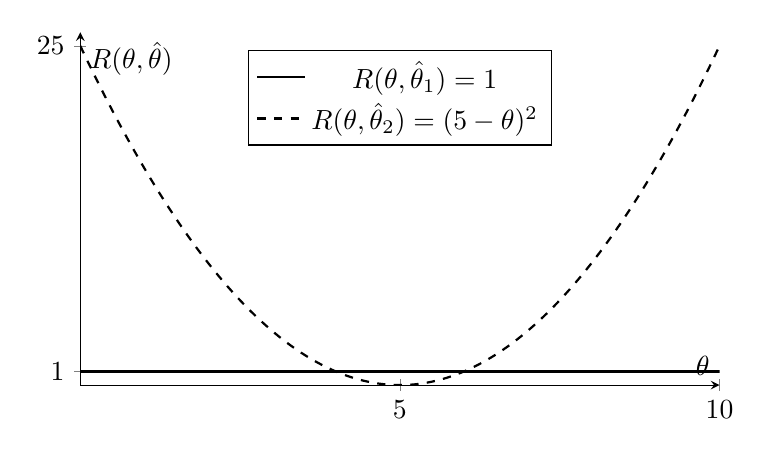
\begin{tikzpicture}
	  \begin{axis}[
		domain=0:10,
		samples=200,
		axis lines=middle,
		xlabel={$\theta$},
		ylabel={$R(\theta,\hat{\theta})$},
		xmin=0, xmax=10,
		ymin=0, ymax=26,
		xtick={0,5,10},
		ytick={0,1,25},
		legend style={at={(0.5,0.95)},anchor=north},
		width=0.8\textwidth,
		height=0.5\textwidth,
	  ]
		% R(theta, \hat{\theta}_1) = 1
		\addplot[thick] {1};
		\addlegendentry{$R(\theta,\hat{\theta}_1)=1$}

		% R(theta, \hat{\theta}_2) = (5 - theta)^2
		\addplot[thick, dashed] {(5 - x)^2};
		\addlegendentry{$R(\theta,\hat{\theta}_2)=(5-\theta)^2$}
	  \end{axis}
	\end{tikzpicture}
	\caption{Risk functions for $\hat{\theta}_1 = X$ and $\hat{\theta}_2 = 5$ under squared error loss.}
	\end{figure}

	Neither estimator wins everywhere. How do we pick between them?
\end{ex}

\begin{defn}[Maximum Risk]
	Define \[
		\overline{R}(\hat{\theta}) = \max_\theta R(\theta, \hat{\theta})
	.\] 
\end{defn}
\begin{defn}[Minimax estimator]
	The minimax estimator is the estimator $\hat{\theta}$ satisfying \[
		\overline{R}(\hat{\theta}) = \inf_{\tilde{\theta}} \overline{R}(\hat{\theta})
	.\] 
\end{defn}

This estimator comes from the frequentist view.

Recall that we have a prior that we are free to use.

\begin{defn}[Bayes Risk (Integrated Risk)]
	Define the Bayes Risk \[
		r(\hat{\theta}) = \int_{}^{} R(\theta, \hat{\theta}) \pi(\theta) d\theta 
	.\] 
\end{defn}
\begin{defn}[Bayes estimator]
	The Bayes estimator associated with a loss function $L$ and a prior $\pi$ is $\hat{\theta}$ such that \[
		r(\hat{\theta}) = \inf_{\tilde{\theta}}r(\tilde{\theta})
	.\] 
\end{defn}

\begin{ex}
	Consider $X\sim \operatorname{Bin}(n, \theta)$ with the prior $\pi(\theta)$ that is uniform on $[0,1]$. We use the square error loss function.

	Suppose we want to compare the two esimators\marginnote{$\hat{\theta}_2$ is the posterior for a $\operatorname{Beta}(\alpha, \beta)$ prior.} \[
		\hat{\theta}_1 = \frac{X}{n}, \quad \hat{\theta}_2 = \frac{\alpha+X}{\alpha+\beta+X}
	.\] 
	
	We can compute
	\begin{align*}
		R(\theta, \hat{\theta}_1) &= \E\left[\left( \hat{\theta}-\theta \right)^2\right]  \\
								 &= \operatorname{Var}\left(\hat{\theta}_1\right) \\
								 &= \frac{\theta(1-\theta)}{n} \\
		\overline{R}(\hat{\theta}_1) &\overbrace{=}^{\theta = \frac{1}{2}} \frac{1}{4n} \\
								 r(\hat{\theta}_1) &= \int_{0}^{1} \frac{\theta(1-\theta)}{n} \cdot  1 d\theta  \\
												   &= \frac{1}{6n} \\
								 R(\theta, \hat{\theta}_2) &= \frac{n \theta(1-\theta) + \left( \alpha - \left( \alpha + \beta \right)\theta \right)^2}{\left( \alpha+\beta+n \right)^2}
	.\end{align*}
	We could maximize and integrate this to find $\overline{R}, r$, since this is just a quadratic in $\theta$. But if we put $\alpha = \beta = \frac{\sqrt{n} }{2}$ for simplicity in just our calculation here, we get 
	\begin{align*}
		R(\theta, \hat{\theta})_2) &= \frac{n}{4 \left( n + \sqrt{n}  \right)^2}  = r(\hat{\theta}_2)
	,\end{align*}
	where we see that since $R$ does not depend on $\theta$, $r$ is immediate.
	Thus, $\hat{\theta}_2$ wins according to the maximum risk decision rule (if our prior is $\alpha = \beta = \frac{\sqrt{n} }{2} $).\marginnote{While this result is surprising, it is because $\hat{\theta}_2$ may be better because of a small part of the sample space.} Meanwhile, for large $n$, $\hat{\theta}_1$ has lower Bayes risk.

	As an extension, the best Bayes estimator ends up being $\hat{\theta}_2 = \frac{\alpha + X}{\alpha + \beta + X}$ with $\alpha = \beta =1$, so \[
		r(\hat{\theta}_2^{1,1}) = \frac{1}{6(n+2)}
	,\] 
	which is the posterior mean.
\end{ex}

The last result is interesting: is the best Bayes estimator always the posterior mean?

\begin{defn}[Posterior risk]
	Define the posterior risk \[
		r(\hat{\theta} \mid X) = \int_{}^{} L(\theta, \hat{\theta}) \pi(\theta \mid X) d\theta
	\] for $X \in \R^n$ that represents the data.
\end{defn}

\begin{thm}
	Let $\hat{\theta} = \hat{\theta}(X)$ be the value that minimizes the posterior risk. Then $\hat{\theta}$ is the Bayes estimator.
\end{thm}
\begin{proof}
	With well behaved functions so Fubini's theorem applies,
	\begin{align*}
		r(\hat{\theta}) &= \int_{}^{} R(\theta, \hat{\theta})\pi(\theta)d\theta  \\
		&= \int_{}^{} \int_{}^{} L(\theta, \hat{\theta}) \underbrace{f(X\mid \theta) \pi(\theta)}_{} dXd\theta		  \\
		&= \int_{}^{} \int_{}^{} L(\theta, \hat{\theta}) \overbrace{\pi(\theta \mid X) f(X) }^{} d\theta dX \\
		&= \int_{}^{} r(\hat{\theta} \mid X) f(X) dX 
	.\end{align*}
\end{proof}

\begin{thm}
	Bayes estimators are:
	\begin{itemize}
		\item square loss $\implies$ posterior mean 
		\item absolute loss $\implies$ posterior median 
		\item zero-one loss $\implies$ posterior mode
	\end{itemize}
\end{thm}
\begin{proof}
	\newthought{(Square loss)} Suppose $X$ is a random variable with mean $\mu$. Then 
	\begin{align*}
		\E\left[\left( X-c \right)^2\right] &= \E\left[\left( x-\mu + \mu - c \right)^2\right] \\
		&= \E\left[\left( x-\mu \right)^2\right] + \left( \mu-c \right)^2
	\end{align*} 
	is minimized at $c=\mu$.
	We write
	\begin{align*}
		r(\hat{\theta}\mid X) = \int_{}^{} \left( \theta - \hat{\theta} \right)^2 \pi(\theta \mid X)d\theta 
	\end{align*}
	and see that is is minimized for $\hat{\theta}$ being the posterior mean.
\end{proof}

\texthl{This is useful because if we want to find the Bayes estimator under one of these three loss functions, we can just find the posterior then find the mean/median/mode.}










\end{document}
